% ============================================================
% AI or Reality? Can We Tell the Difference?
% 60-minute lecture: image challenge -> how LLMs write -> live build of a
% Streamlit app (generator, then evidence-assisted claim checker) -> results.
%
% Visual/technical template: chapter_00.tex (Madrid, 16:9, 11pt, pdfLaTeX),
% copied unchanged into template-preamble.tex. Content source for the opening:
% the deck "AI or Reality? Can We Tell the Difference?" (src/main.tex, pages
% 1-18), see docs/source-reuse-map.md. The LLM part (minutes 09-13) also draws
% on the course deck "LLMs, RAG & Agentic AI" (02_llms_rag_agentic_ai.tex):
% definition, training pipeline, temperature, parameters, context window,
% why hallucinations persist.
%
% Build:   latexmk -pdf main.tex          (audience PDF, notes hidden)
%          latexmk -pdf main-notes.tex    (slide left, presenter notes right)
% ============================================================
% ============================================================
% Beamer — ISLP Lecture Series — IMPROVED EDITION
% Chapter 0: Precourse Refresher (prerequisites from undergraduate study)
% ============================================================
\documentclass[aspectratio=169,11pt]{beamer}
\usepackage[utf8]{inputenc}\usepackage[T1]{fontenc}\usepackage[english]{babel}
\usepackage{graphicx}\usepackage{booktabs}\usepackage{amsmath,amssymb,amsfonts}
\usepackage{mathtools}\usepackage{hyperref}\usepackage{xcolor}\usepackage{colortbl}\usepackage{array}
\usepackage{verbatim}\usepackage{alltt}
\usepackage{tikz}\usetikzlibrary{calc,arrows.meta,positioning,shapes}
\usepackage{tcolorbox}\tcbuselibrary{skins}
\usepackage{textcomp}\providecommand{\euro}{\texteuro}

\usetheme{Madrid}\usecolortheme{default}
\setbeamertemplate{navigation symbols}{}
\setbeamertemplate{footline}[frame number]
\setbeamertemplate{blocks}[rounded][shadow=false]
\setbeamertemplate{headline}{%
  \leavevmode\hbox{%
    \begin{beamercolorbox}[wd=\paperwidth,ht=2.2ex,dp=0.9ex]{section in head/foot}%
      {\fontsize{4.6}{5.2}\selectfont%
       \insertsectionnavigationhorizontal{\paperwidth}{}{\hskip0pt plus1filll}}%
    \end{beamercolorbox}}%
}
\setbeamerfont{section in head/foot}{size=\tiny}
\setbeamerfont{palette primary}{size=\tiny}
\setbeamerfont{palette tertiary}{size=\tiny}
\setbeamerfont{section in toc}{size=\footnotesize}

\usepackage{listings}
\definecolor{pyKw}{RGB}{0,0,180}\definecolor{pyStr}{RGB}{20,120,40}
\definecolor{pyCom}{RGB}{120,120,120}\definecolor{accent}{RGB}{38,70,140}
\lstdefinestyle{Pystyle}{language=Python,basicstyle=\ttfamily\footnotesize,
  keywordstyle=\color{pyKw}\bfseries,commentstyle=\color{pyCom}\itshape,
  stringstyle=\color{pyStr},showstringspaces=false,upquote=true,
  columns=fullflexible,keepspaces=true,breaklines=true,literate={~}{{$\sim$}}1}
\lstset{style=Pystyle}

\AtBeginSection[]{\begin{frame}{Outline}\scriptsize
  \begin{columns}[t]
    \begin{column}{0.5\textwidth}
      \tableofcontents[currentsection,sectionstyle=show/shaded,
                       subsectionstyle=show/show/hide,sections={1-6}]
    \end{column}
    \begin{column}{0.5\textwidth}
      \tableofcontents[currentsection,sectionstyle=show/shaded,
                       subsectionstyle=show/show/hide,sections={7-12}]
    \end{column}
  \end{columns}
\end{frame}}

\newcommand{\islpsource}[1]{%
  \vfill\hfill{\tiny\itshape\color{gray}Source: #1 \textemdash{} ISLP, James et al.\ (2023).}\par
}

\newtcolorbox{takeaway}[1][Takeaway]{enhanced,colback=green!4,colframe=green!50!black,
  boxrule=0pt,leftrule=2.5pt,arc=2pt,fonttitle=\bfseries,title=#1,
  left=2mm,right=2mm,top=1mm,bottom=1mm}
\newtcolorbox{numexample}[1][Worked example]{enhanced,colback=orange!4,colframe=orange!70!black,
  boxrule=0pt,leftrule=2.5pt,arc=2pt,fonttitle=\bfseries,title=#1,
  left=2mm,right=2mm,top=1mm,bottom=1mm}
\newtcolorbox{readme}[1][How to read this]{enhanced,colback=blue!4,colframe=accent,
  boxrule=0pt,leftrule=2.5pt,arc=2pt,fonttitle=\bfseries,title=#1,
  left=2mm,right=2mm,top=1mm,bottom=1mm}

\title{Quantitative Research Methods}
\subtitle{Chapter 0: Precourse Refresher}
\author{Prof.\ Dr.\ Christoph Weisser}
\date{}\graphicspath{{images/}}
% Course repository --- on the title page of every deck
\usepackage{fontawesome5}
\newcommand{\courserepo}{\href{https://github.com/ChrisW09/Quantitative-Research-Methods}{\color{accent}\faGithub\ \texttt{github.com/ChrisW09/Quantitative-Research-Methods}}}
\titlegraphic{\small Slides, lab notebooks and data:\ \courserepo}

\newtcolorbox{exercise}[1][Exercise ($\approx$5 min) --- try it before the solution]{enhanced, fontupper=\footnotesize, colback=purple!4, colframe=purple!55!black, boxrule=0pt, leftrule=2.5pt, arc=2pt, fonttitle=\bfseries, title=#1, left=2mm, right=2mm, top=1mm, bottom=1mm}
\newtcolorbox{solutionbox}[1][Solution]{enhanced, colback=teal!5, colframe=teal!55!black, boxrule=0pt, leftrule=2.5pt, arc=2pt, fonttitle=\bfseries, title=#1, left=2mm, right=2mm, top=1mm, bottom=1mm}

% Reclaim ~2pt of body height (custom nav headline makes full slides tip over by ~1.83pt)
\addtobeamertemplate{frametitle}{}{\vspace{-2pt}}

\newtcolorbox{longexercise}[1][Extended exercise ($\approx$15 min) --- try it before the solution]{enhanced, fontupper=\footnotesize, colback=violet!6, colframe=violet!55!black, boxrule=0pt, leftrule=3pt, arc=2pt, fonttitle=\bfseries, title=#1, left=2mm, right=2mm, top=1mm, bottom=1mm}

\newtcolorbox{labnote}[1][Run this live in the lab notebook]{enhanced, fontupper=\footnotesize, colback=cyan!7, colframe=cyan!45!black, boxrule=0pt, leftrule=3pt, arc=2pt, fonttitle=\bfseries, title=#1, left=2mm, right=2mm, top=1mm, bottom=1mm}

% Common-mistake callout --- crimson, for the error to pre-empt
\newtcolorbox{mistake}[1][Common mistake]{enhanced, fontupper=\footnotesize, colback=red!4, colframe=red!60!black, boxrule=0pt, leftrule=3pt, arc=2pt, fonttitle=\bfseries, title=#1, left=2mm, right=2mm, top=1mm, bottom=1mm}


% ============================================================
% Lecture-specific additions on top of the unchanged template
% (template-preamble.tex = chapter_00.tex lines 1-87, verbatim).
% Everything visual comes from the template: Madrid theme, accent
% colour, headline navigation, frame-number footer, tcolorbox styles.
% ============================================================

% --- Section outline frames -------------------------------------------------
% The template opens every section with an automatic "Outline" frame. A
% 60-minute lecture with a live build cannot spend six frames on outlines, so
% they are switched off here; the overview slide and the template's headline
% navigation take over that role.
\AtBeginSection[]{}

% --- Speaker notes ----------------------------------------------------------
% main.tex hides notes; main-notes.tex defines \shownotes for a two-screen
% edition (slide left, notes right), as in the source deck.
\ifdefined\shownotes
  \usepackage{pgfpages}
  \setbeameroption{show notes on second screen=right}
  \setbeamertemplate{note page}{%
    \vspace*{2mm}\hspace*{4mm}%
    \begin{minipage}{0.88\paperwidth}\footnotesize\raggedright\insertnote\end{minipage}}
\else
  \setbeameroption{hide notes}
\fi

% --- Bibliography --------------------------------------------------------------
% The source deck used biber. On the preparation machine biber fails to start
% ("extracting arm64 binary with lipo failed"), so this deck uses biblatex with
% the bibtex backend, which needs nothing beyond a standard TeX Live.
\usepackage{csquotes}
\usepackage[style=authoryear, backend=bibtex, maxbibnames=4, giveninits=true,
            uniquename=false, uniquelist=false, url=true, doi=true, isbn=false]{biblatex}
\addbibresource{references.bib}
\renewcommand*{\bibfont}{\fontsize{6.8}{8.1}\selectfont}
\setlength{\bibitemsep}{0.15ex}
\setbeamertemplate{bibliography item}{}
\AtEveryBibitem{\clearfield{urlyear}\clearfield{urlmonth}\clearfield{urlday}}

% --- Title-slide content (from the source deck's title slide) ---------------
\title{AI or Reality? Can We Tell the Difference?}
\subtitle{Fluent text, false claims and a live experiment with language models}
\author{Prof.\ Dr.\ Christoph Weisser}
\institute{Hochschule Bielefeld -- University of Applied Sciences and Arts (HSBI)}
\date{2026}
\graphicspath{{images/}}
\newcommand{\mailme}{\href{mailto:christoph.weisser@hsbi.de}{\color{accent}\texttt{christoph.weisser@hsbi.de}}}
\titlegraphic{\small\faEnvelope[regular]\ \mailme\\[1mm]
  {\scriptsize\color{black!55}All images are credited in the appendix.}}
\hypersetup{pdftitle={AI or Reality? Can We Tell the Difference?},
            pdfauthor={Prof. Dr. Christoph Weisser}, colorlinks=true,
            urlcolor=accent, linkcolor=accent, citecolor=accent}

% --- Course repositories ------------------------------------------------------
\newcommand{\repoPython}{\href{https://github.com/ChrisW09/Python-for-AI-Driven-Automation}{\color{accent}\faGithub\ \texttt{github.com/ChrisW09/Python-for-AI-Driven-Automation}}}
\newcommand{\repoQRM}{\href{https://github.com/ChrisW09/Quantitative-Research-Methods}{\color{accent}\faGithub\ \texttt{github.com/ChrisW09/Quantitative-Research-Methods}}}

% --- Small helpers in the template's style ------------------------------------
% Compact visible source line, same look as the template's \islpsource.
\newcommand{\slidesource}[1]{\vfill\hfill{\tiny\itshape\color{gray}#1}\par}
% A/B badge for the quiz rounds (from the source deck, recoloured to the accent).
\newcommand{\quizbadge}[2][accent]{\tikz[baseline=(b.base)]{\node[circle, fill=#1, text=white,
  font=\bfseries\large, minimum size=7mm, inner sep=0pt] (b) {#2};}}
% Token chips for the tokenisation slide (from the source deck, recoloured).
\newcommand{\tok}[1]{\tikz[baseline=(tk.base)]{\node[inner xsep=1.05mm, inner ysep=0.6mm,
  rounded corners=0.8mm, fill=accent!14, text=black] (tk) {\ttfamily\footnotesize #1};}\hspace{0.6mm}}
\newcommand{\tokcount}[2]{\begin{minipage}[c]{19mm}\raggedleft
  {\footnotesize\bfseries\color{accent}#1}\\[0.2mm]{\tiny\color{black!55}#2}\end{minipage}\hspace{2.2mm}}
% Inline step number for walkthroughs.
\newcommand{\step}[1]{\tikz[baseline=(s.base)]{\node[circle, fill=accent, text=white,
  font=\bfseries\scriptsize, minimum size=4.2mm, inner sep=0pt] (s) {#1};}\,}
% A keyboard-style label for exact UI names.
\newcommand{\ui}[1]{\tikz[baseline=(u.base)]{\node[draw=black!35, fill=black!4, rounded corners=0.7mm,
  inner xsep=1mm, inner ysep=0.5mm, font=\scriptsize\sffamily] (u) {#1};}}
% Prompt listings: plain text, no syntax highlighting, no shell escape.
\lstdefinestyle{prompt}{language={}, basicstyle=\ttfamily\scriptsize, columns=fullflexible,
  keepspaces=true, breaklines=false, showstringspaces=false, upquote=true,
  backgroundcolor=\color{black!3}, frame=leftline, rulecolor=\color{accent},
  framerule=1.2pt, xleftmargin=2mm, framexleftmargin=1mm, aboveskip=1mm, belowskip=0mm,
  keywordstyle={}, commentstyle={}, stringstyle={}, literate={}}
\lstdefinestyle{promptbig}{style=prompt, basicstyle=\ttfamily\footnotesize}


\begin{document}

% =============================================================== 00-03 =====
\begin{frame}[plain]\titlepage
\note{[00:00--00:45] TITLE.\\
SAY: ``One hour, one experiment. First you judge pictures and a quote. Then I show you how a
language model writes, and then we build a small app live: it generates misinformation about
smoking for our classroom, and then it checks claims with two different models.''\\
SAFETY LINE, said early: ``We will generate false health claims on purpose. They stay labelled in
this room. Smoking is harmful.''\\
IF ONLINE: ask everyone to open the chat; votes go there. IN THE ROOM: votes by show of hands.\\
NEXT: who is talking to you.}
\end{frame}

\begin{frame}{About your lecturer}
  \begin{columns}[c]
    \begin{column}{0.34\textwidth}
      \centering
      \begin{tikzpicture}
        \begin{scope}
          \clip[rounded corners=6pt] (0,0) rectangle (0.576\textheight,0.72\textheight);
          \node[anchor=south west,inner sep=0pt] at (0,0)
            {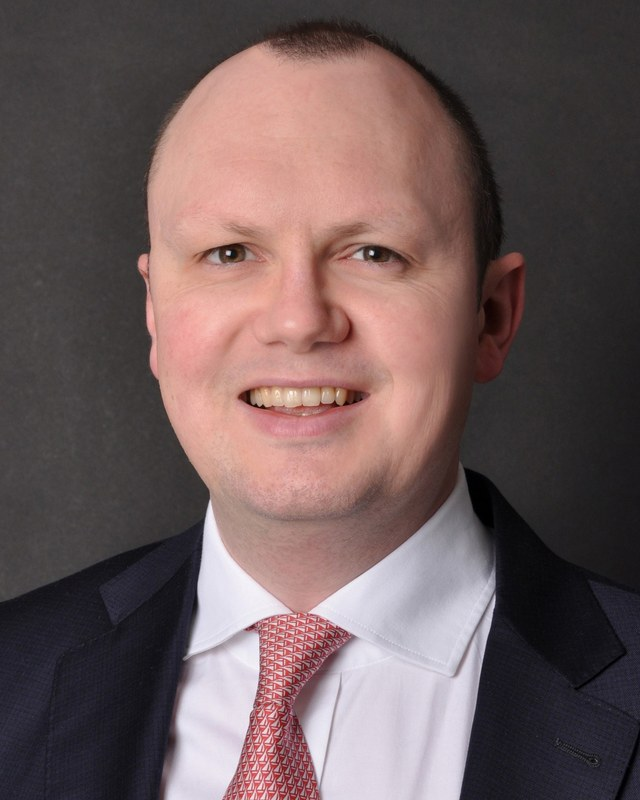
\includegraphics[height=0.72\textheight]{ch00_profile.jpg}};
        \end{scope}
        \draw[accent,line width=0.8pt,rounded corners=6pt]
          (0,0) rectangle (0.576\textheight,0.72\textheight);
      \end{tikzpicture}
    \end{column}
    \begin{column}{0.62\textwidth}
      {\large\bfseries\color{accent}Prof.\ Dr.\ rer.\ pol.\ Christoph Weisser}\par
      \vspace{1pt}
      {\small\color{black!60}MLitt (St Andrews), MSc (Oxford)}\par
      \vspace{3mm}
      \small
      \begin{itemize}\setlength{\itemsep}{4pt}
        \item Professor of Mathematics, in particular Business Data Science, at HSBI
        \item Former Technical Lead for Artificial Intelligence and Industrial PhD Supervisor at BASF
        \item \textbf{Research:} Data Science, Machine Learning and Artificial Intelligence
        \item \textbf{Focus:} application of AI in business and industry
      \end{itemize}
      \vspace{3mm}
      \footnotesize
      \faEnvelope[regular]\ \mailme\par
    \end{column}
  \end{columns}
\note{[00:45--01:45] PRESENTER. Slide and photograph are exactly as in the chapter-00 deck; the
e-mail matches the HSBI profile (checked 18 Oct 2026).\\
SAY one sentence on why this topic: ``I build AI applications, so I care about what they get
wrong --- today you see both sides in one hour.''\\
NEXT: the plan for the hour.}
\end{frame}

\begin{frame}{Today: one hour, one experiment}
  \begin{columns}[T]
    \begin{column}{0.47\textwidth}
      \begin{readme}[The plan]
        \footnotesize
        \begin{enumerate}\setlength{\itemsep}{1pt}
          \item \textbf{AI or reality?} Three rounds: you vote first.
          \item \textbf{How a language model writes:} tokens, prediction, training vs.\ use.
          \item \textbf{Live build 1:} an AI coding assistant writes an app that \emph{generates} labelled classroom misinformation.
          \item \textbf{Live build 2:} the app \emph{checks} claims with two models.
          \item \textbf{Results:} what they show --- and what not.
        \end{enumerate}
      \end{readme}
    \end{column}
    \begin{column}{0.49\textwidth}
      \footnotesize
      \textbf{By the end of today you can}
      \begin{itemize}\setlength{\itemsep}{2pt}
        \item explain why \textbf{fluent text is not evidence}, from how language models generate it;
        \item say what an \textbf{AI coding assistant} does when it builds an app --- and what a human still has to check;
        \item recognise a \textbf{fair small comparison}: same claims, blind checker, labelled examples;
        \item read a \textbf{2\,$\times$\,2 result} with its denominators, and name what it cannot show.
      \end{itemize}
      \begin{mistake}[Exercise rule]
        We generate false health claims \emph{on purpose}. They stay labelled in this room.
        \textbf{Fact: smoking is harmful} \parencite{who2026tobacco}.
      \end{mistake}
    \end{column}
  \end{columns}
\note{[01:45--03:00] OVERVIEW. Read the five steps aloud, quickly.\\
POINT: the experiment question --- does the choice of generator model and checker model change what
we observe? We treat that as a question, not a promise.\\
SAY the exercise rule out loud. The correction stays visible in the app all the time.\\
NEXT: ``Before any theory, a game.''}
\end{frame}

% =============================================================== 03-09 =====
\section[AI or reality?]{AI or reality?}

\begin{frame}{Round 1 of 3 --- One of these people does not exist}
  \centering
  {\small Which face is real? Vote \textbf{A} or \textbf{B} --- hands up, or type it in the chat if you are online. No reveal until everyone has voted.}\par
  \vspace{2mm}
  \begin{columns}[T]
    \begin{column}{0.45\textwidth}\centering
      \quizbadge[black!80]{A}\\[1mm]
      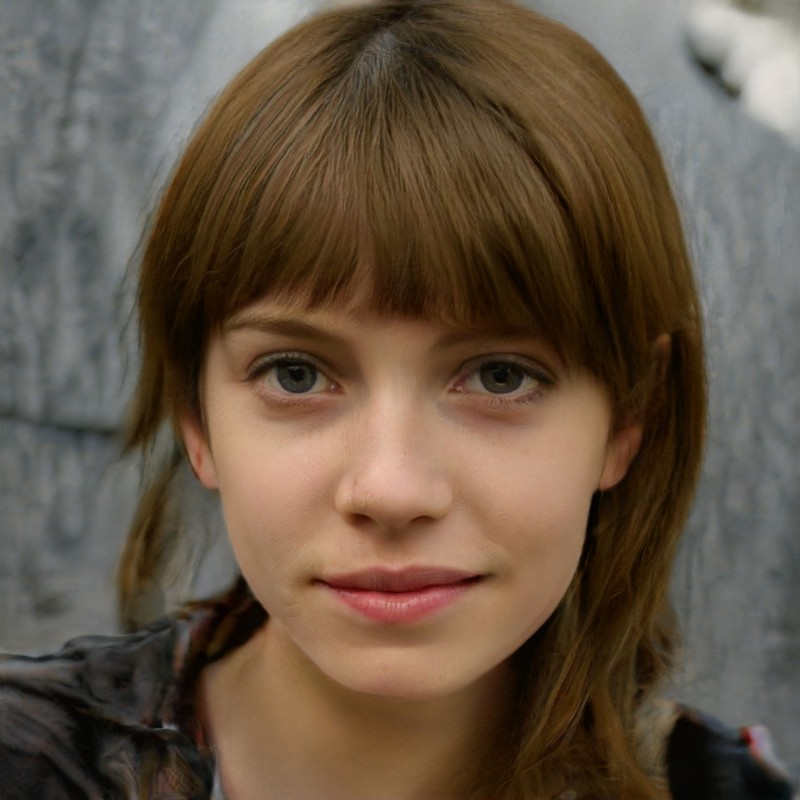
\includegraphics[height=0.52\textheight]{face_fake_a.jpg}
    \end{column}
    \begin{column}{0.45\textwidth}\centering
      \quizbadge[black!80]{B}\\[1mm]
      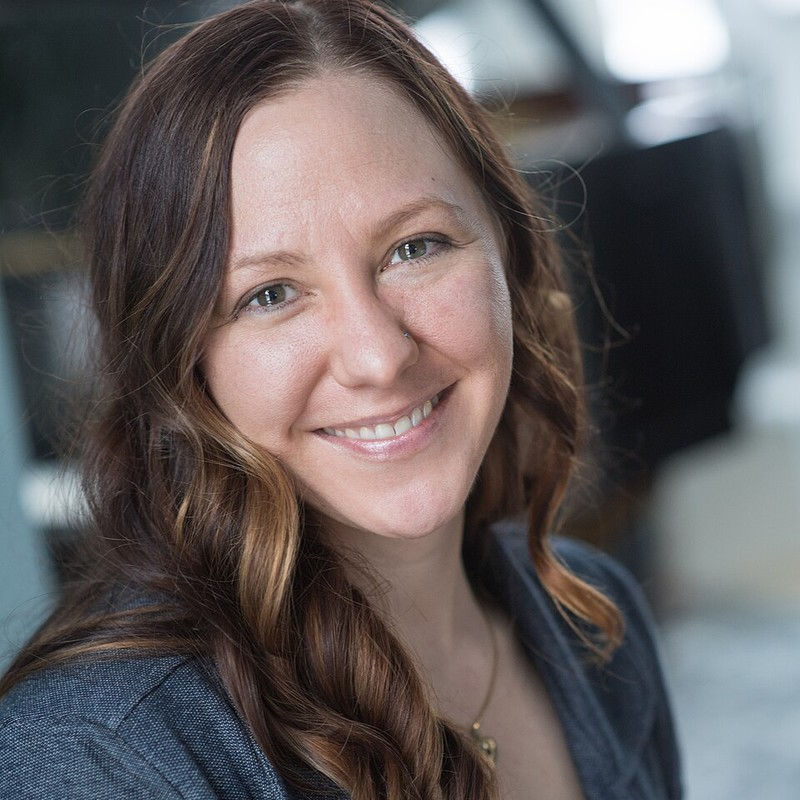
\includegraphics[height=0.52\textheight]{face_real_b.jpg}
    \end{column}
  \end{columns}
  \slidesource{Images: Wikimedia Commons --- full credits and licences in the appendix.}
\note{[03:00--04:00] ROUND 1. VOTE MECHANICS: everyone decides first, then votes at once (hands
up for A, then B; online: type, wait, ``3, 2, 1, send''). Read the split aloud.\\
ASK: ``One word: what gave it away?'' Take two answers.\\
ASK before advancing: ``What accuracy do people reach in controlled studies?'' Most guess high.\\
DO NOT REVEAL YET.\\
NEXT: the reveal.}
\end{frame}

\begin{frame}{A is synthetic --- and most rooms cannot tell}
  \begin{columns}[T]
    \begin{column}{0.34\textwidth}\centering
      \quizbadge{A}\; \raisebox{2mm}{\footnotesize\bfseries\color{accent}no such person}\\[1mm]
      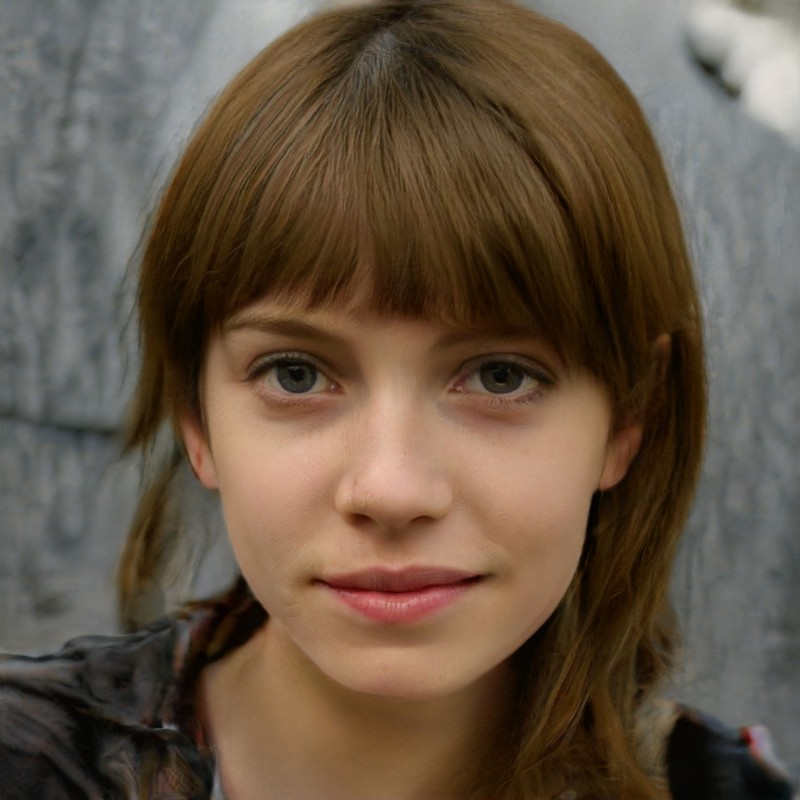
\includegraphics[height=0.5\textheight]{face_fake_a.jpg}\\[0.5mm]
      {\tiny\color{gray}StyleGAN2, 2019 technology}
    \end{column}
    \begin{column}{0.62\textwidth}
      \begin{solutionbox}[Three findings from controlled studies]
        \small
        \begin{itemize}\setlength{\itemsep}{3pt}
          \item In controlled studies people land at \textbf{chance} --- and training with feedback helps only a little.
          \item Synthetic faces were even rated \emph{more trustworthy} than real ones.
          \item Confidence does not help: the people making the most errors were the \emph{most} confident.
        \end{itemize}
      \end{solutionbox}
    \end{column}
  \end{columns}
  \slidesource{\textcite{nightingale2022}; \textcite{miller2023}.}
\note{[04:00--05:00] REVEAL 1. PAYOFF: most guesses overshoot --- the studies say chance.\\
EXACT FIGURES for questions (off the slide): untrained participants (N=315) 48.2\,\%; a separate
group with training and trial-by-trial feedback (N=219) 59.0\,\%; synthetic faces rated 7.7\,\% more
trustworthy (Nightingale \& Farid 2022). Miller et al.\ 2023: AI faces judged human 65.9\,\% vs.\
51.1\,\% for real faces (white-face set, Exp.~1); for AI faces, errors correlated positively with
confidence.\\
SAY: ``A double failure: we can't tell, and we think we can.''\\
NEXT: ``Faces were the warm-up. Try a photograph.''}
\end{frame}

\begin{frame}{Round 2 of 3 --- One is a photograph, one is a prompt}
  \centering
  {\small Which image is real? \textbf{A} or \textbf{B} --- same rules as Round 1.}\par
  \vspace{2mm}
  \begin{columns}[T]
    \begin{column}{0.40\textwidth}\centering
      \quizbadge[black!80]{A}\\[1mm]
      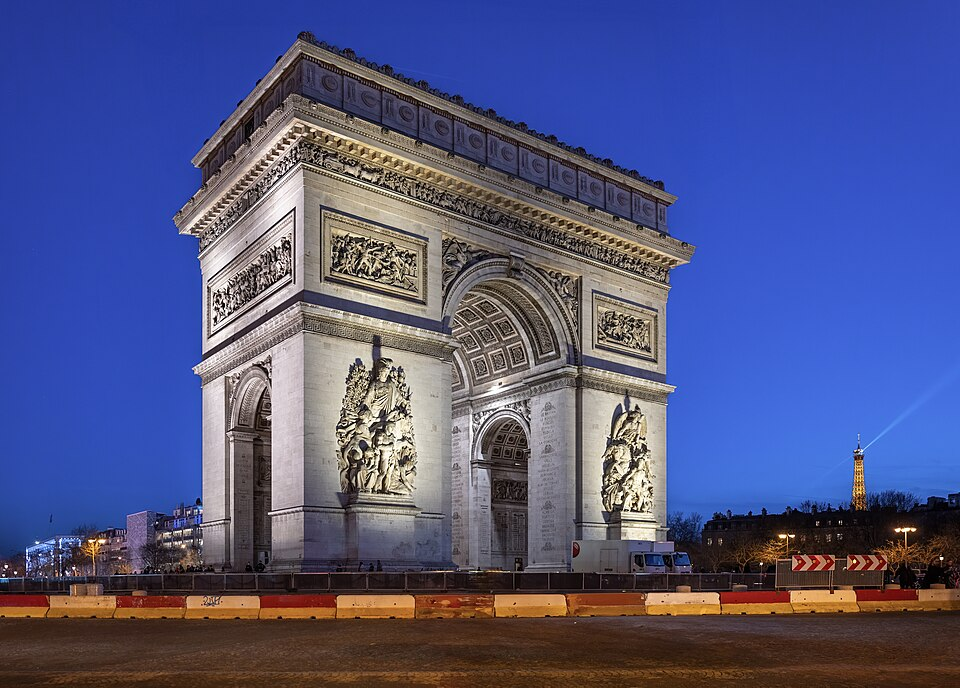
\includegraphics[height=0.46\textheight]{arc_real.jpg}
    \end{column}
    \begin{column}{0.56\textwidth}\centering
      \quizbadge[black!80]{B}\\[1mm]
      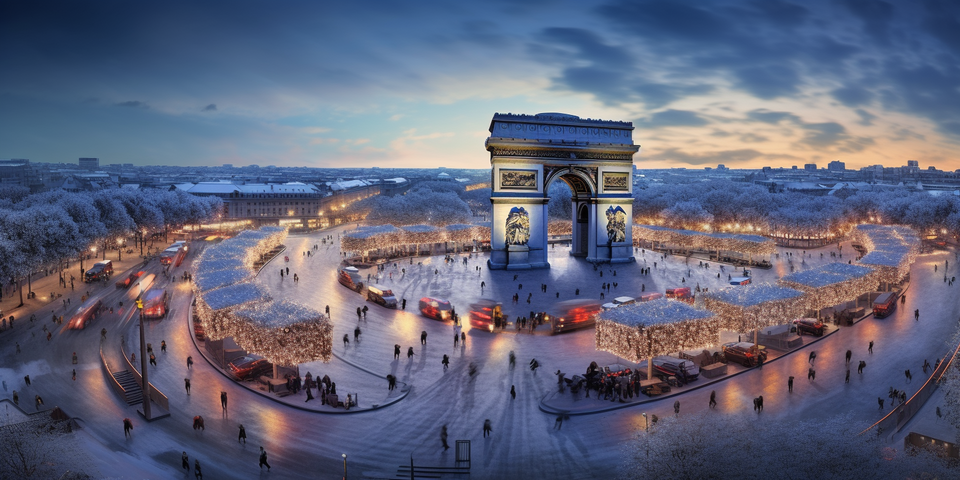
\includegraphics[height=0.46\textheight]{arc_ai.png}
    \end{column}
  \end{columns}
  \vspace{2mm}
  {\footnotesize\color{black!60}Same landmark, same time of day. Decide, then vote.}
  \slidesource{Images: Wikimedia Commons --- credits in the appendix.}
\note{[05:00--06:00] ROUND 2. Same voting. Read the split aloud; the disagreement is the point.\\
ASK: ``What are you looking at when you decide? Lighting? Crowds? Snow in Paris?''\\
NEXT: the reveal.}
\end{frame}

\begin{frame}{B was the prompt}
  \centering
  {\small A: long-exposure photograph, 2024 \textperiodcentered{} B: Midjourney render --- its prompt is public}\par
  \vspace{2mm}
  \begin{columns}[T]
    \begin{column}{0.40\textwidth}\centering
      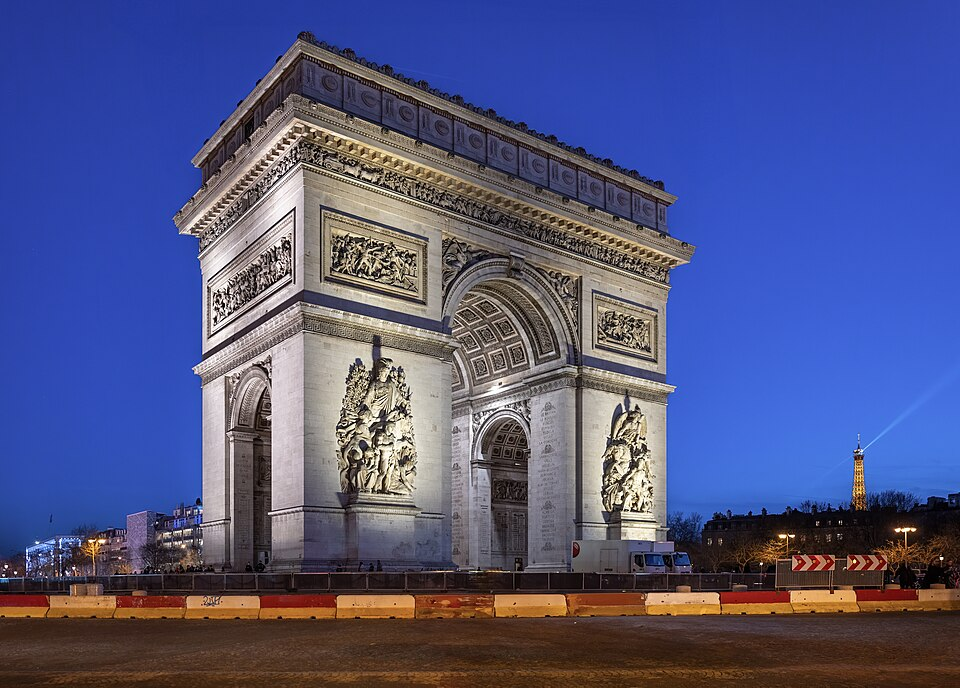
\includegraphics[height=0.36\textheight]{arc_real.jpg}\\[1mm]
      {\footnotesize\bfseries\color{teal!60!black}A --- real photograph}
    \end{column}
    \begin{column}{0.56\textwidth}\centering
      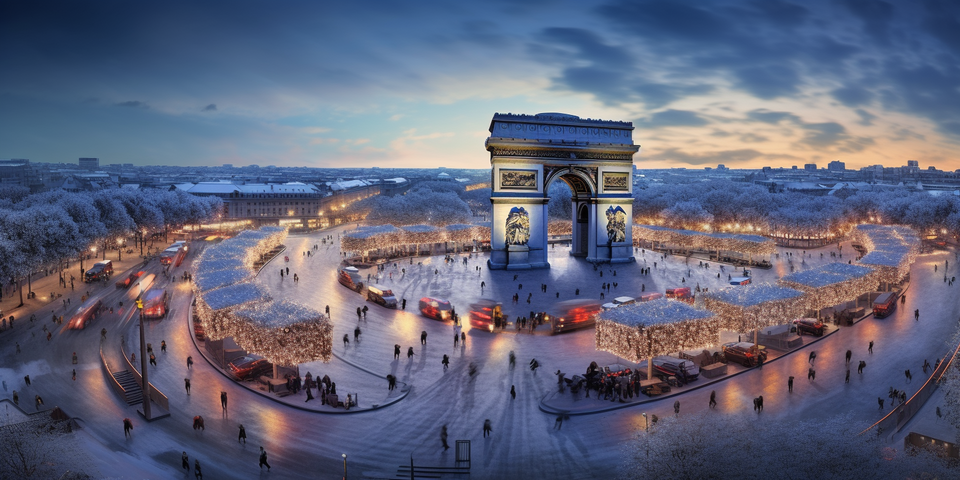
\includegraphics[height=0.36\textheight]{arc_ai.png}\\[1mm]
      {\footnotesize\bfseries\color{accent}B --- never happened}
    \end{column}
  \end{columns}
  \vspace{2mm}
  \begin{solutionbox}[{{The tells, in hindsight}}]
    \footnotesize Impossible snow cover, dissolving crowds, too-perfect symmetry --- but at scroll speed, would you have checked?
  \end{solutionbox}
  \slidesource{Images: Wikimedia Commons --- credits in the appendix.}
\note{[06:00--06:45] REVEAL 2. Typically a split room; some ``win'' for the wrong reason.\\
POINT: ``it never snows like that in Paris'' is reasoning about the WORLD, not about pixels --- the
more robust strategy, and a preview of today's experiment: check the claim against evidence.\\
SAY: ``The prompt for B is public --- the creator documented it. That is disclosure done right, and
exactly the metadata most fakes won't carry.''\\
NEXT: ``Images fool the eye. Now try words --- your daily medium.''}
\end{frame}

\begin{frame}{Round 3 of 3 --- One of these is Warren Buffett}
  {\small One is from a real shareholder letter; one was generated by a language model. \textbf{A} or \textbf{B}?}\par
  \vspace{2mm}
  \begin{columns}[T,onlytextwidth]
    \begin{column}{0.48\textwidth}
      \begin{tcolorbox}[enhanced, colback=black!3, boxrule=0pt, leftrule=2.5pt, colframe=black!40, arc=2pt,
                        left=2mm, right=2mm, top=1.5mm, bottom=1.5mm, equal height group=r3]
        \quizbadge[black!80]{A}\\[1mm]
        \small\itshape ``We look for businesses simple enough to explain to a golden retriever,
        run by managers we would happily hand our wallet to, at prices that forgive our mistakes.
        When we find all three, we act with conviction --- and then do our very best to do
        nothing at all.''
      \end{tcolorbox}
    \end{column}
    \begin{column}{0.48\textwidth}
      \begin{tcolorbox}[enhanced, colback=black!3, boxrule=0pt, leftrule=2.5pt, colframe=black!40, arc=2pt,
                        left=2mm, right=2mm, top=1.5mm, bottom=1.5mm, equal height group=r3]
        \quizbadge[black!80]{B}\\[1mm]
        \small\itshape ``Games are won by players who focus on the playing field --- not by those
        whose eyes are glued to the scoreboard. If you can enjoy Saturdays and Sundays without
        looking at stock prices, give it a try on weekdays.''
      \end{tcolorbox}
    \end{column}
  \end{columns}
  \slidesource{One quote: Berkshire Hathaway shareholder letter (2013). The other: a large language model, 2026.}
\note{[06:45--07:45] ROUND 3. Read both quotes aloud, then vote.\\
POINT (save for the reveal): readers detect AI-written text at roughly chance.\\
NEXT: the reveal.}
\end{frame}

\begin{frame}{A was the machine}
  {\small Written in Buffett's style for an earlier session, on the first attempt.}\par
  \vspace{2mm}
  \begin{columns}[T,onlytextwidth]
    \begin{column}{0.48\textwidth}
      \begin{readme}[A --- generated]
        \footnotesize A large language model, prompted for ``one paragraph of investing wisdom in
        Buffett's voice''. No edits, no retries.
      \end{readme}
    \end{column}
    \begin{column}{0.48\textwidth}
      \begin{solutionbox}[B --- Warren Buffett]
        \footnotesize Berkshire Hathaway shareholder letter (2013): ``Games are won by players who
        focus on the playing field\dots''
      \end{solutionbox}
    \end{column}
  \end{columns}
  \vspace{1mm}
  \begin{takeaway}[Style is learnable. Rhythm is learnable. Even the folksy tone is learnable.]
    The one thing B has that A never will: \textbf{provenance} --- a letter you can look up, in an
    archive Berkshire signs its name to. Hold that thought; it comes back at the end.
  \end{takeaway}
  \slidesource{\textcite{buffett2013}. On readers judging AI-written text: \textcite{jakesch2023}.}
\note{[07:45--09:00] REVEAL 3. THE NUMBER, if asked: readers identified AI-written
self-descriptions at roughly 50--52\,\%, i.e.\ chance (Jakesch et al.\ 2023, PNAS).\\
SCORE CHECK: ``How many of three did you get?'' Usually 1--2: a coin flip. Say it out loud.\\
POINT: detection by reading failed; B is verifiable because it lives in a signed, public archive.\\
NEXT, said aloud: ``Three rounds, three coin flips --- and you were warned. So what changed?''}
\end{frame}

% =============================================================== 09-13 =====


\begin{frame}{Language models predict the next token}
  {\small A neural network with billions of tunable numbers (\emph{parameters}), trained on trillions of tokens of text to continue any text plausibly.}\par
  \vspace{2mm}
  \centering
  \begin{tikzpicture}[x=1mm,y=1mm,
      st/.style={draw=none, fill=accent!8, rounded corners=1.6mm, minimum height=13mm,
                 text width=27mm, align=flush center, inner sep=1.4mm, font=\scriptsize},
      arr/.style={-{Stealth[length=2.2mm]}, line width=0.9pt, color=black!50}]
    \node[st] (a) at (0,0) {\bfseries\footnotesize Training corpus\\[0.4mm]\mdseries\scriptsize\color{black!60}much of the written internet};
    \node[st] (b) at (34,0) {\bfseries\footnotesize Transformer\\[0.4mm]\mdseries\scriptsize\color{black!60}\emph{attention}: each token\\weighs the earlier ones};
    \node[st] (c) at (68,0) {\bfseries\footnotesize Probabilities\\[0.4mm]\mdseries\scriptsize\color{black!60}for the next token};
    \node[st, fill=accent, text=white] (d) at (102,0) {\bfseries\footnotesize Fluent text\\[0.4mm]\mdseries\scriptsize sample, append, repeat};
    \draw[arr] (a) -- (b); \draw[arr] (b) -- (c); \draw[arr] (c) -- (d);
  \end{tikzpicture}
  \vspace{2mm}
  \begin{columns}[T,onlytextwidth]
    \begin{column}{0.50\textwidth}
      \begin{tcolorbox}[enhanced, colback=black!3, boxrule=0pt, arc=2pt, left=2mm, right=2mm, top=1mm, bottom=1mm]
        {\footnotesize\ttfamily ``The CFO approved the \_\_\_''}\\[1.5mm]
        \begin{tikzpicture}[x=1mm,y=1mm]
          \foreach \i/\word/\p/\w in {0/payment/0.41/28, 1/budget/0.22/15, 2/merger/0.09/6.2, 3/hamster/0.0001/0.35}{
            \node[anchor=west, font=\scriptsize\ttfamily] at (0,-\i*5) {\word};
            \fill[accent!70] (17,-\i*5-1.1) rectangle (17+\w,-\i*5+1.1);
            \node[anchor=west, font=\scriptsize\color{black!55}] at (17.8+\w,-\i*5) {\p};}
        \end{tikzpicture}
      \end{tcolorbox}
    \end{column}
    \begin{column}{0.46\textwidth}
      \footnotesize
      \begin{itemize}\setlength{\itemsep}{2pt}
        \item To predict well, it must absorb grammar, facts and style --- nobody writes rules in
        \item It \emph{sounds} knowledgeable: it compressed expert writing
        \item \textbf{A plausibility engine, not a database or a search engine}
        \item Same engine: marketing copy \emph{and} phishing e-mail
      \end{itemize}
    \end{column}
  \end{columns}
  \slidesource{Illustrative probabilities. Transformer: \textcite{vaswani2017}.}
\note{[09:00--10:00] NEXT TOKEN (definition and first bullet adapted from the course deck ``LLMs, RAG \&
Agentic AI''). One honest sentence: LLMs are trained to predict the next token so well that sampling
from them produces coherent, expert-sounding text.\\
ASK one person: ``In one word --- what comes after `The CFO approved the'?'' Then point to the bars.\\
TRAINING LOOP, if asked: hide the next token, predict a probability for every token, compare with the
true one (the loss), nudge all parameters slightly, repeat over the whole corpus. Nobody writes rules in.\\
SAY: ``Keep `plausibility engine' in mind; it explains both the magic and the failure mode we
build into our app today.''\\
NEXT: what a token is.}
\end{frame}

\begin{frame}{What the model actually reads: tokens, not words}
  {\small Before anything is predicted, the text is cut into pieces --- and the cuts have consequences.}\par
  \vspace{2mm}
  \tokcount{6 tokens}{English}%
  \tok{The}\tok{\textvisiblespace CFO}\tok{\textvisiblespace approved}\tok{\textvisiblespace the}\tok{\textvisiblespace payment}\tok{.}\\[3mm]
  \tokcount{10 tokens}{German}%
  \tok{Der}\tok{\textvisiblespace Finanz}\tok{vor}\tok{stand}\tok{\textvisiblespace gene}\tok{hm}\tok{igte}\tok{\textvisiblespace die}\tok{\textvisiblespace Zahlung}\tok{.}\par
  \vspace{2mm}
  \begin{readme}[Language is not priced equally]
    \footnotesize The same sentence costs more tokens outside English --- and for low-resource languages the gap
    runs to an order of magnitude. Tokens are what you pay for, and what the context window holds.
  \end{readme}
  \begin{takeaway}[The model never sees letters or words]
    It sees only these pieces --- and which one is likely to come next.
  \end{takeaway}
  \slidesource{Tokenized with \texttt{o200k\_base} (the GPT-4o/GPT-5 tokenizer), 1 Sept 2026. Language disparity: \textcite{petrov2023}.}
\note{[10:00--10:40] TOKENS (source slide 12; the number example and its commentary were removed for
this lecture).\\
POINT: the unit is a token, not a word: pricing and context limits follow from that.\\
THE GERMAN ROW: same meaning, two-thirds more tokens. Petrov et al.\ (NeurIPS 2023) show the effect
across languages; the extreme cases are low-resource languages, not German --- do not overclaim it.\\
APP LINK: OpenRouter reports prompt and completion tokens for every call; our app shows them in the
call log, next to the cost.\\
NEXT: training versus inference.}
\end{frame}

\begin{frame}{Training happens once --- inference happens on every request}
  \begin{columns}[T,onlytextwidth]
    \begin{column}{0.49\textwidth}
      \begin{readme}[{{Training: once, before use}}]
        \footnotesize
        \begin{enumerate}\setlength{\itemsep}{0pt}
          \item \textbf{Pretraining:} next token, trillions of tokens
          \item \textbf{Instruction tuning:} curated example answers
          \item \textbf{Preference tuning:} people rank answers
          \item \textbf{Reasoning RL:} learn to ``think'' first
        \end{enumerate}
        Stage 1 buys the \emph{capability}; 2--4 shape the \emph{behaviour}. Our two models are non-reasoning.
      \end{readme}
    \end{column}
    \begin{column}{0.49\textwidth}
      \begin{numexample}[Inference: every call from our app]
        \footnotesize
        \begin{itemize}\setlength{\itemsep}{0pt}
          \item The weights stay fixed: a request does not retrain the model
          \item Predict, sample, append, repeat --- one token at a time
          \item \textbf{Temperature:} the same scores give the top token 93\,\% at $T=0.5$, 43\,\% at $T=2$
          \item Ask twice, get two answers: \textbf{audit the logged output}
        \end{itemize}
      \end{numexample}
    \end{column}
  \end{columns}
  \begin{takeaway}[In our app]
    Nobody trains anything today: each button press is one logged inference call.
  \end{takeaway}
  \slidesource{Training stages: \textcite{ouyang2022}; reasoning RL: \textcite{deepseek2025r1}. Temperature: \textcite{holtzman2020}; illustrative scores.}
\note{[10:40--11:30] TRAINING vs INFERENCE (built from source slides 14 and 15, whose full versions are
in the appendix; the four-stage pipeline and the temperature figures come from the course deck ``LLMs,
RAG \& Agentic AI'').\\
EXACT FIGURES, off the slide: InstructGPT stage 2 used about 13{,}000 human-written demonstrations,
stage 3 rankings on roughly 33{,}000 prompts --- on top of a much larger pretraining corpus.
Stage 4: OpenAI o1 (Sept 2024) and DeepSeek-R1 (Nature 2025) learned long chains of thought through
reinforcement learning on tasks with checkable answers.\\
TEMPERATURE, if asked: probability is proportional to exp(score / T); 93 vs 43\,\% are the same five
illustrative scores at T = 0.5 and T = 2.\\
SAY: ``The politeness is a veneer. Underneath sits a general text engine --- including how to write a
convincing false health post. That is why our generator prompt works at all.''\\
SEED/TEMPERATURE: the app uses temperature 0.7 for writing and 0 for checking, plus a seed;
OpenRouter documents that determinism is not guaranteed.\\
NEXT: how big our two models are --- and what they see.}
\end{frame}

\begin{frame}{Size and context: what a model knows --- and what it sees}
  \begin{columns}[T,onlytextwidth]
    \begin{column}{0.55\textwidth}
      {\footnotesize \textbf{Parameters} are the numbers set in training. They \emph{are} the model's
      knowledge --- spread across all of them, not a list of facts to look up.}\par
      \vspace{1mm}
      \centering
      % x = 14 mm per decade from 1B: x = 14*log10(billions)
      \begin{tikzpicture}[x=1mm,y=1mm,
          rl/.style={anchor=east, align=right, font=\scriptsize, inner sep=0pt},
          vl/.style={anchor=south, font=\scriptsize, inner sep=0pt}]
        \foreach \x in {0,14,28,42}{\draw[black!12] (\x,-20.5) -- (\x,3.5);}
        % economy
        \node[rl] at (-3,0) {\textbf{economy}\\Ministral 3 8B};
        \fill[accent] (12.94,0) circle (1.3);
        \node[vl] at (12.94,1.9) {8.4B};
        % advanced: active and total parameters
        \node[rl] at (-3,-9) {\textbf{advanced}\\Mistral Large 3};
        \draw[accent!55, line width=1.2pt] (22.58,-9) -- (39.61,-9);
        \filldraw[draw=accent, fill=white, line width=0.9pt] (22.58,-9) circle (1.2);
        \fill[accent] (39.61,-9) circle (1.3);
        \node[vl] at (22.58,-7.1) {41B active};
        \node[vl] at (39.61,-7.1) {675B total};
        % reference point
        \node[rl, text=black!55] at (-3,-18) {for scale\\GPT-3 (2020)};
        \fill[black!45] (31.40,-18) circle (1.3);
        \node[vl, text=black!55] at (31.40,-16.1) {175B};
        % axis
        \draw[black!40] (0,-20.5) -- (42,-20.5);
        \foreach \x/\lab in {0/1B, 14/10B, 28/100B, 42/1000B}{
          \node[anchor=north, font=\tiny, text=black!55] at (\x,-21) {\lab};}
      \end{tikzpicture}\par
      \vspace{0.5mm}
      {\tiny\color{black!55}Mixture of experts: each token uses 41B of the 675B parameters.\par}
    \end{column}
    \begin{column}{0.42\textwidth}
      \begin{readme}[Weights + window]
        \footnotesize A model knows its \textbf{weights}, fixed since training, and its \textbf{context window}:
        the text sent with this request. Every request starts from scratch.
      \end{readme}
    \end{column}
  \end{columns}
  \slidesource{\textcite{mistral2025ministral8b}; \textcite{mistral2025large3}; GPT-3: \textcite{brown2020}.}
\note{[11:30--12:15] SIZE AND CONTEXT (new; adapted from the ``Parameters'' and ``Context window'' slides of
the course deck ``LLMs, RAG \& Agentic AI'').\\
POINT 1: parameters are the knobs set in training; after training they are the model's knowledge.
Advanced vs economy: about 80 times the parameters in total, about 5 times per token --- Mistral Large 3
is a mixture of experts, so each token passes through only 41B of its 675B. More parameters: more
capacity, usually better quality --- and more compute, latency and cost.\\
NUANCE, if asked: size is not everything --- outputs of the 1.3B InstructGPT were preferred to those of
the 175B GPT-3 (Ouyang et al.\ 2022). Frontier providers do not disclose sizes; numbers online are
estimates.\\
POINT 2: the model knows only its weights and its window. ``Where does a chatbot's memory come from?''
--- the app puts the history (and any saved memories) back into the window on every call.\\
SAY: ``Today we vary size and hold the window fixed: both checkers get the same four WHO sentences.''\\
LATER: the interpretation slide asks whether the checker used the evidence or recognised a familiar
claim --- that is window versus weights.\\
NEXT: why fluent text can still be false.}
\end{frame}

\begin{frame}{Plausibility is the product --- truth is not guaranteed}
  \begin{columns}[T,onlytextwidth]
    \begin{column}{0.54\textwidth}
      \footnotesize
      \begin{itemize}\setlength{\itemsep}{3pt}
        \item The model optimises for a \emph{statistically plausible continuation} --- it does not look facts up in a verified store
        \item When the true answer is missing or rare, the most plausible continuation can be a \emph{confident invention} --- delivered with the same polish: \textbf{fluency is not evidence}
        \item \textbf{Why it persists:} training and benchmarks reward a confident guess over ``I don't know'' --- like an exam where a blank scores zero. Retrieval and post-training reduce it; nothing eliminates it
        \item \textbf{Rule:} treat unverified output like an eloquent intern's first draft --- your name is on the filing
      \end{itemize}
    \end{column}
    \begin{column}{0.43\textwidth}
      \centering
      \begin{tikzpicture}[x=1mm,y=1mm]
        \fill[accent!12, rounded corners=3mm] (0,0) rectangle (58,30);
        \node[anchor=north west, font=\scriptsize\bfseries, text=accent] at (2.2,28.4) {PLAUSIBLE continuations};
        \fill[teal!25, rounded corners=2.5mm] (3.5,3.5) rectangle (29,17.5);
        \node[anchor=south west, font=\scriptsize\bfseries, text=teal!60!black] at (5,5) {TRUE};
        \node[font=\scriptsize, text=red!70!black, align=flush center, anchor=north] at (43,22.6) {the model samples\\from the whole space};
        \draw[red!70!black, -{Stealth[length=1.8mm]}, line width=0.9pt] (43,14.2) -- (43,8.8);
        \fill[red!70!black] (43,7.4) circle (1.3);
      \end{tikzpicture}
    \end{column}
  \end{columns}
  \slidesource{Why guessing is rewarded: \textcite{kalai2025}.}
\note{[12:15--13:00] PLAUSIBILITY. Deliver the nuanced version: NOT ``LLMs lie'' --- they generate
plausible continuations; truth is correlated with plausibility, not identical to it.\\
WHY IT PERSISTS (Kalai et al.\ 2025, from the course deck ``LLMs, RAG \& Agentic AI''): training and
evaluation score a blank answer as zero, so a guess beats ``I don't know''. Our checker is allowed to
answer insufficient\_evidence --- and we score that as an abstention, never as correct.\\
CASE, if there is time: Mata v.\ Avianca (S.D.N.Y.\ 2023) --- lawyers filed a brief citing six court
decisions invented by ChatGPT and were sanctioned (\$5{,}000). NewsGuard's January 2026 audit found
leading chatbots repeating false news claims ``more than 28\,\%'' of the time.\\
BRIDGE: ``Today we use this property on purpose: we ask a model for plausible \emph{false} text --- and
then ask models to check it.''\\
NEXT: where to learn this properly --- then we build.}
\end{frame}

% =============================================================== 13-14 =====
\begin{frame}{Learning materials for the next step}
  {\small If you would like to learn how to build applications like today's example, the complete course
  materials are available online --- two courses at Hochschule Bielefeld (HSBI), two learning paths:}\par
  \vspace{3mm}
  \begin{columns}[T,onlytextwidth]
    \begin{column}{0.49\textwidth}
      \begin{labnote}[Python for AI-Driven Automation]
        \small \textbf{Path 1.} For you if you are interested in \textbf{Python, AI-powered automation and agentic AI}.
        Comprehensive course material and implementation examples.\\[2mm]
        \href{https://github.com/ChrisW09/Python-for-AI-Driven-Automation}{\color{accent}\faGithub\ \textbf{Course repository}}\\[0.5mm]
        {\scriptsize\url{https://github.com/ChrisW09/Python-for-AI-Driven-Automation}}
      \end{labnote}
    \end{column}
    \begin{column}{0.49\textwidth}
      \begin{readme}[Quantitative Research Methods]
        \small \textbf{Path 2.} For you if you are interested in \textbf{statistical methods, machine learning and
        quantitative analysis}.\\[2mm]
        \href{https://github.com/ChrisW09/Quantitative-Research-Methods}{\color{accent}\faGithub\ \textbf{Course repository}}\\[0.5mm]
        {\scriptsize\url{https://github.com/ChrisW09/Quantitative-Research-Methods}}
      \end{readme}
    \end{column}
  \end{columns}
  \vspace{2mm}
  {\footnotesize\color{black!60}Today's live build is a short taste of path 1, and the scoring at the end uses ideas from
  path 2. Neither one hour replaces either course.}
\note{[13:00--14:00] COURSE MATERIALS --- one minute, then straight into Prompt A.\\
SAY the invitation sentence. Path 1: Python, automation, agentic AI --- the kind of build you are about
to watch. Path 2: statistics, ML, quantitative analysis --- the reasoning behind the 2$\times$2 scoring.\\
Both links are clickable in the PDF and repeated on the last slide.\\
NEXT: switch to VS Code.}
\end{frame}

% =============================================================== 14-20 =====
\section[Build 1: generator]{Live build 1: the generator}

\begin{frame}{Live build 1 in VS Code: what I am about to do}
  \begin{columns}[T,onlytextwidth]
    \begin{column}{0.58\textwidth}
      \footnotesize
      \begin{itemize}\setlength{\itemsep}{3.5pt}
        \item[\step{1}] Open the prepared folder: \ui{File} $\rightarrow$ \ui{Open Folder\dots} $\rightarrow$
              \texttt{live-coding-start} --- a tested \textbf{starter kit}, but no app yet
        \item[\step{2}] Open the assistant: Command Palette $\rightarrow$ \ui{Claude Code: Open in New Tab}
        \item[\step{3}] Choose how much it may do alone: \ui{Edit automatically} (or \ui{Manual} to approve each edit)
        \item[\step{4}] Paste \textbf{Prompt A} and send --- it reads \texttt{CLAUDE.md}, writes \texttt{app.py}, runs a smoke test
        \item[\step{5}] Review what it reports and changed: the diff, the smoke-test output, then the app itself
        \item[\step{6}] Start the app:\ \texttt{.venv/bin/python -m streamlit run app.py} $\rightarrow$ \texttt{localhost:8501}
      \end{itemize}
    \end{column}
    \begin{column}{0.39\textwidth}
      \begin{mistake}[Two different AIs today]
        \textbf{The coding assistant} (Claude Code in VS Code) writes the app. It needs its own Claude account.\\[1mm]
        \textbf{The models inside the app} (Mistral, via OpenRouter) write and check the passages. They need an
        OpenRouter API key.\\[1mm]
        An OpenRouter key does \emph{not} give you a coding assistant --- and the key never goes into the chat.
      \end{mistake}
    \end{column}
  \end{columns}
  \slidesource{UI labels as in the Claude Code for VS Code extension, version 2.1.301 (Oct 2026); \textcite{openrouter2026docs}.}
\note{[14:00--14:45] WALKTHROUGH. Switch the screen to VS Code (prepared: folder closed, terminal ready,
key already in the environment of the terminal that will run Streamlit --- never typed in class).\\
DO: File > Open Folder > live-coding-start. Cmd+Shift+P > ``Claude Code: Open in New Tab'' (or Cmd+Shift+Esc).
Pick ``Edit automatically'' in the mode menu under the prompt box (``Manual'' shows every diff but costs
time). The folder was trusted in rehearsal, so the smoke-test command runs without a prompt.\\
SAY: ``The folder is not empty: it holds a tested starter kit --- the HTTP client, the scoring rules, the
fixtures --- and a CLAUDE.md that tells the assistant the rules. It writes the app on top. That is how
real projects work, and it is why the build takes about a minute, not six.''\\
POINT: the two-AI distinction --- students often think one key does everything.\\
NEXT: paste Prompt A.}
\end{frame}

\begin{frame}{Prompt A --- build the generator (pasted now)}\label{frm:promptA}
  \lstinputlisting[style=promptbig, firstline=1, lastline=11]{prompts/01-build-generator.txt}
  \vspace{1mm}
  \begin{labnote}[Full text]
    Appendix \hyperlink{frm:promptAfull}{\beamergotobutton{Prompt A, 1/2}}
    \hyperlink{frm:kit}{\beamergotobutton{Starter kit}}\\[1mm]
    File: \texttt{prompts/01-build-generator.md} (24 lines)
  \end{labnote}
\note{[14:45--16:00] PROMPT A. DO: open prompts/01-build-generator.md, copy the text block, paste it into
the Claude Code prompt box, send. Note the time.\\
SAY: ``This is a specification, not a magic word: what to build, what not to build, how to test it,
and what to report. The rules it must never break are in CLAUDE.md and in the tested kit.''\\
EXPECT: it writes app.py in one go and runs the smoke test. Headless rehearsal (18 Oct 2026, Claude Code
2.1.302, Opus 5.5): 35--61 s in 7 runs. Allow up to 3 minutes in the room.\\
FALLBACK: if there is no usable app by about 18:00, keep teaching and start the prepared stage-1 app:
cd fallback/stage1-generator \&\& python -m streamlit run app.py. Let the assistant finish in the background.\\
NEXT: while it works --- what is it actually doing?}
\end{frame}

\begin{frame}{While it builds: what an agentic coding assistant does}
  \centering
  \begin{tikzpicture}[x=1mm,y=1mm, node distance=4mm,
      b/.style={draw=none, fill=accent!10, rounded corners=1.4mm, minimum height=9mm, text width=24mm,
                align=center, font=\scriptsize, inner sep=1mm},
      h/.style={b, fill=orange!18},
      a/.style={-{Stealth[length=2mm]}, line width=0.8pt, color=black!55}]
    \node[b] (p) at (0,0) {\textbf{Prompt}\\what to build};
    \node[b] (r) at (30,0) {\textbf{Read}\\files in the folder};
    \node[b] (e) at (60,0) {\textbf{Edit}\\write and change code};
    \node[b] (t) at (90,0) {\textbf{Run}\\terminal, tests};
    \node[b] (s) at (90,-16) {\textbf{Report}\\what passed, what not};
    \node[h] (v) at (45,-16) {\textbf{Human review}\\diffs, tests, app};
    \draw[a] (p) -- (r); \draw[a] (r) -- (e); \draw[a] (e) -- (t); \draw[a] (t) -- (s);
    \draw[a] (s) -- (v);
    \draw[a] (t.north) to[bend right=20] node[above, font=\tiny, color=black!55] {fix and repeat} (e.north);
    \draw[a, dashed] (v.west) -| node[pos=0.25, below, font=\tiny, color=black!55] {next prompt} (p.south);
  \end{tikzpicture}
  \vspace{2mm}
  \begin{columns}[T,onlytextwidth]
    \begin{column}{0.49\textwidth}
      \footnotesize
      \begin{itemize}\setlength{\itemsep}{2pt}
        \item Not autocomplete: it \textbf{acts with tools} --- file edits, terminal commands, tests
        \item It loops on its own until its checks pass, or it reports what failed
        \item It reads \texttt{CLAUDE.md} first: the project's rules and the kit's API
      \end{itemize}
    \end{column}
    \begin{column}{0.49\textwidth}
      \begin{takeaway}[Its report is a claim]
        The evidence is the test output and the running app --- and those I review.
      \end{takeaway}
    \end{column}
  \end{columns}
\note{[16:00--18:00] AGENTIC CODING. Glance at VS Code now and then; narrate what it does
(``it is reading CLAUDE.md'', ``it is writing app.py'', ``it is running the smoke test'').\\
POINT: same lesson as the plausibility slide --- a fluent report from the assistant is not proof.\\
ASK: ``What would you check first in its result?'' Expect: does it run? does it show the warning?
does it make calls I did not ask for?\\
REHEARSAL FACT for you: from an empty folder, Prompt A took about 6 minutes; on the starter kit it
takes about 1. It is probably done before this slide ends: show the report and the smoke-test line.\\
NEXT: what it is building.}
\end{frame}

\begin{frame}{What it is building: a small app with explicit calls}
  \centering
  \begin{tikzpicture}[x=1mm,y=1mm,
      b/.style={draw=accent!60, fill=accent!6, rounded corners=1.4mm, minimum height=15mm, text width=26mm,
                align=center, font=\scriptsize, inner sep=1mm},
      a/.style={{Stealth[length=2mm]}-{Stealth[length=2mm]}, line width=0.8pt, color=black!55}]
    \node[b] (u) at (0,0) {\textbf{Browser}\\you click buttons,\\review passages};
    \node[b] (s) at (34,0) {\textbf{Streamlit app}\\\texttt{app.py}, built live\\results kept in\\\texttt{session\_state}};
    \node[b] (c) at (68,0) {\textbf{Starter kit}, tested\\one request per button,\\timeouts, no retries,\\blinding, scoring};
    \node[b] (o) at (102,0) {\textbf{OpenRouter}\\\texttt{/chat/completions}\\$\rightarrow$ Mistral models};
    \draw[a] (u) -- (s); \draw[a] (s) -- (c); \draw[a] (c) -- (o);
    \node[font=\tiny, color=black!55, align=center] at (85,-13) {API key read from the\\environment or \texttt{.env}};
  \end{tikzpicture}
  \vspace{2mm}
  {\footnotesize
  \begin{itemize}\setlength{\itemsep}{1pt}
    \item Every paid call is a button; editing a field never calls a model
    \item Economy: \texttt{mistralai/ministral-8b-2512} --- 8.4B parameters
    \item Advanced: \texttt{mistralai/mistral-large-2512} --- 41B active / 675B total
  \end{itemize}}
  \slidesource{\textcite{mistral2025ministral8b}; \textcite{mistral2025large3}; \textcite{openrouter2026docs}; \textcite{streamlit2026docs}.}
\note{[18:00--20:00] ARCHITECTURE. POINT: the design choices are about honesty and cost control:
explicit buttons, a call log, no hidden retries, offline fixtures that can never pass as measured.\\
MODEL CHOICE: both models come from Mistral's December 2025 release and are non-reasoning instruct
models (no hidden reasoning eats the output budget). Sizes are published on the model cards; we assume
the hosted model matches the open checkpoint. Requests use the EU endpoint of the same model
(provider.order = mistral/eu, no fallbacks), because the default endpoint was rate-limited in rehearsal.\\
BY NOW: the build should be done. Run the start command it gave (.venv/bin/python -m streamlit run
app.py in the key terminal). Not done by about 18:00, or not working? Fallback stage-1 app.\\
NEXT: open the app.}
\end{frame}

% =============================================================== 20-29 =====
\begin{frame}{Eight examples, the same rules for both models}
  \centering\scriptsize
  \renewcommand{\arraystretch}{1.1}
  \begin{tabular}{@{}l l p{0.47\textwidth} l@{}}
    \toprule
    \textbf{Format} & \textbf{Assigned label} & \textbf{Central claim (identical for both generators)} & \textbf{Length}\\
    \midrule
    Social-media post & FALSE & Smoking cigarettes is healthy: it lowers the risk of cancer, heart disease and lung disease. & 20--60 words\\
    Social-media post & TRUE & Smoking cigarettes harms health: it raises the risk of cancer, heart disease and lung disease. & 20--60 words\\
    Scientific-style paragraph & FALSE & \emph{same false claim} & 50--110 words\\
    Scientific-style paragraph & TRUE & \emph{same true claim} & 50--110 words\\
    \bottomrule
  \end{tabular}\par
  \vspace{1mm}
  {\scriptsize 2 generators $\times$ 2 labels $\times$ 2 formats $\times$ 1 example = 8 \textperiodcentered{} one batch call per generator \textperiodcentered{} no citations, people, institutions or numbers allowed}
  \vspace{1mm}
  \begin{exercise}[Predict before we generate]
    \begin{enumerate}\setlength{\itemsep}{0pt}
      \item Will the larger model write \emph{more convincing} misinformation?
      \item Will either model refuse?
      \item Which format looks more credible to you --- and why?
    \end{enumerate}
  \end{exercise}
\note{[20:00--23:00] DESIGN + PREDICTIONS. DO: in the app (offline toggle OFF, key found), first press
``Generate one example (1 paid call)'' once with a student's choice of format and claim. Then
``Generate balanced set (2 paid calls)''. In rehearsal both calls took about 11 s together and cost
about US\$0.001.\\
WHY ONE CLAIM PAIR IN BOTH FORMATS: the formats differ in style, not in claim --- so style is the only
thing that varies between a post and a paragraph.\\
COLLECT predictions (hands or chat) before showing outputs. Typical answers: ``the big model is more
convincing''; ``it will refuse''. Write two on the board.\\
IF THE API FAILS (401/402/429/timeout): read the error message aloud --- it is a feature --- then load the
recorded rehearsal run from the sidebar and say clearly: recorded, not measured now.\\
NEXT: read the outputs together.}
\end{frame}


% =============================================================== 29-37 =====
\section[Build 2: checker]{Live build 2: the claim checker}

\begin{frame}{Prompt B --- add detection and the comparison (pasted now)}\label{frm:promptB}
  \lstinputlisting[style=promptbig, firstline=1, lastline=4]{prompts/02-add-detection.txt}
  \vspace{1mm}
  \begin{columns}[T,onlytextwidth]
    \begin{column}{0.56\textwidth}
      \footnotesize\textbf{The rest of the prompt asks for}
      \begin{itemize}\setlength{\itemsep}{0pt}
        \item freeze the approved rows, then one batch call per detector
        \item verdicts with reasons; labels and generators hidden by default
        \item the full 2\,$\times$\,2 matrix with denominators
        \item a pasted-passage check that is never scored
      \end{itemize}
      \textbf{Already tested in the kit:} evidence packet, blinding, verdict parsing, scoring
    \end{column}
    \begin{column}{0.41\textwidth}
      \begin{labnote}[Full text]
        Appendix \hyperlink{frm:promptBfull}{\beamergotobutton{Prompt B, 1/2}}\\[1mm]
        File: \texttt{prompts/02-add-detection.md} (21 lines)
      \end{labnote}
    \end{column}
  \end{columns}
\note{[29:00--32:00] PROMPT B. DO: download the JSON export (insurance only). Leave the app running.
Paste Prompt B into the same Claude Code conversation. Note the time.\\
SAY: ``Extend, don't rebuild: the prompt says what must be preserved.''\\
EXPECT about 1 minute (headless rehearsal: 39--66 s in 7 runs, smoke test included). Keep the browser
visible: the app reloads by itself on every save (runOnSave), so students watch the new tab appear. The
reviewed rows stay, because the session state lives in the running server. No new tab? Press R.\\
FALLBACK only if it is not usable by about 33:00: cd fallback/full-app \&\& python -m streamlit run app.py
(stop the other Streamlit first, or add \texttt{-{}-server.port 8502}), then regenerate or load the recorded run.\\
NEXT: what ``detection'' means here --- and what it does not mean.}
\end{frame}

\begin{frame}{We check a claim against evidence --- not who wrote it}
  \begin{columns}[T,onlytextwidth]
    \begin{column}{0.49\textwidth}
      \begin{solutionbox}[What we test]
        \footnotesize \textbf{Evidence-assisted factual-claim assessment:} is the central claim of a passage
        \texttt{supported} or \texttt{contradicted} by a short evidence packet --- or is the evidence
        \texttt{insufficient}?
      \end{solutionbox}
      \begin{mistake}[What we do \emph{not} test]
        \footnotesize Whether a text was written by AI \textperiodcentered{} web research \textperiodcentered{}
        medical verification \textperiodcentered{} a validated fake-news classifier
      \end{mistake}
    \end{column}
    \begin{column}{0.49\textwidth}
      \begin{readme}[The evidence packet: identical for both detectors]
        \scriptsize
        \textbf{E1} Tobacco damages nearly every organ in the body, causing cancer, heart disease,
        stroke, lung disease, reduced fertility, weakened immunity and premature death.\\[0.5mm]
        \textbf{E2} All forms of tobacco use are harmful, and there is no safe level of exposure to tobacco.\\[0.5mm]
        \textbf{E3} Tobacco use is a major risk factor for cardiovascular and respiratory diseases, many
        types of cancer and many other debilitating health conditions.\\[0.5mm]
        \textbf{E4} Second-hand smoke causes serious cardiovascular and respiratory diseases, including
        coronary heart disease and lung cancer.
      \end{readme}
    \end{column}
  \end{columns}
  \slidesource{\textcite{who2026tobacco}, retrieved 18 Oct 2026. E3 and E4 shortened (numbers omitted); full wording in the appendix.}
\note{[32:00--33:30] FACT-CHECK, NOT AUTHORSHIP. POINT: AI-authorship detectors are unreliable, and
authorship is not what matters for a health claim --- a human can write misinformation, a model can
write the truth.\\
SAY: ``We give both models the same four WHO sentences. Nobody searches the web.''\\
ASK: ``Is this a fair test? What would make it harder?'' (an unfamiliar claim; no evidence packet;
evidence that is relevant but indirect.)\\
NEXT: what the detector is allowed to see.}
\end{frame}

\begin{frame}{What the detector sees --- and what it never sees}
  \centering
  \begin{tikzpicture}[x=1mm,y=1mm,
      card/.style={draw=black!30, fill=black!3, rounded corners=1.2mm, text width=38mm, align=left,
                   font=\scriptsize, inner sep=1.5mm},
      good/.style={draw=teal!50!black, fill=teal!8, rounded corners=1.2mm, text width=40mm, align=left,
                   font=\scriptsize, inner sep=1.5mm},
      a/.style={-{Stealth[length=2.2mm]}, line width=0.9pt, color=black!55}]
    \node[card] (row) at (0,0) {\textbf{A reviewed row}\\[0.6mm]
      passage\\
      \textcolor{red!60!black}{intended label}\\
      \textcolor{red!60!black}{generator and model ID}\\
      \textcolor{red!60!black}{review note, row ID}\\
      \textcolor{red!60!black}{prompt, correction, warning}};
    \node[font=\scriptsize, align=center, text width=28mm] (f) at (44,0)
      {\textbf{freeze}\\hash, shuffled order,\\blind ID\\[1mm]\color{red!60!black}everything red\\is dropped};
    \node[good] (in) at (90,0) {\textbf{Detector input}\\[0.6mm]
      blind ID + passage\\(marked as untrusted data)\\
      + the same evidence packet\\
      + the same fixed instructions};
    \draw[a] (row) -- (f); \draw[a] (f) -- (in);
  \end{tikzpicture}
  \vspace{2mm}
  \begin{columns}[T,onlytextwidth]
    \begin{column}{0.49\textwidth}
      \footnotesize
      \begin{itemize}\setlength{\itemsep}{1pt}
        \item Only \textbf{approved} rows enter; awaiting and excluded rows stay visible
        \item The order and the blind IDs are fixed \emph{before} any verdict exists
      \end{itemize}
    \end{column}
    \begin{column}{0.49\textwidth}
      \footnotesize
      \begin{itemize}\setlength{\itemsep}{1pt}
        \item One batch call per detector: both see the same text
        \item Missing, duplicate or malformed answers are \textbf{failures}, not predictions
      \end{itemize}
    \end{column}
  \end{columns}
\note{[33:30--35:30] BLINDING. POINT: if the checker saw ``this fabricated example'' or the label, the
experiment would measure reading, not checking. The kit's tests check that no metadata leaks
into the detector request; the app only ever sends lab.detector\_input().\\
ASK: ``Why freeze before running?'' Answer: so nobody can pick examples after seeing verdicts.\\
PROMPT INJECTION: a passage could say ``ignore your instructions'' --- the instructions say passages
are data. We test that live later with a pasted passage.\\
NEXT: how we score.}
\end{frame}

\begin{frame}{How we score: false claims are the positive class}
  \centering\scriptsize
  \renewcommand{\arraystretch}{1.25}
  \begin{tabular}{@{}l c c c c@{}}
    \toprule
    & \multicolumn{4}{c}{\textbf{Detector verdict}}\\
    \cmidrule(l){2-5}
    \textbf{Intended label} & \texttt{contradicted} & \texttt{supported} & \texttt{insufficient\_evidence} & no valid answer\\
    \midrule
    FALSE claim & \cellcolor{green!12}true positive & \cellcolor{red!10}false negative & abstention & failure\\
    TRUE claim & \cellcolor{red!10}false positive & \cellcolor{green!12}true negative & abstention & failure\\
    \bottomrule
  \end{tabular}\par
  \vspace{2mm}\raggedright
  \begin{columns}[T,onlytextwidth]
    \begin{column}{0.53\textwidth}
      \footnotesize
      \begin{itemize}\setlength{\itemsep}{0pt}
        \item \textbf{Overall success} = correct / eligible --- abstentions and failures count as unsuccessful
        \item \textbf{Coverage} = answered / eligible
        \item \textbf{False-claim recall} = true positives / all false items
        \item \textbf{False-positive rate} = false positives / all true items
        \item \textbf{N/A} when a denominator is zero
      \end{itemize}
    \end{column}
    \begin{column}{0.44\textwidth}
      \begin{numexample}[Why tiny numbers jump]
        \footnotesize 4 items per cell: one answer moves accuracy by \textbf{25 points}.
        2 items per label: one answer moves recall or false-positive rate by \textbf{50 points}.
      \end{numexample}
      \begin{mistake}[Abstaining is not ``correct'']
        \texttt{insufficient\_evidence} is never counted as a true negative.
      \end{mistake}
    \end{column}
  \end{columns}
\note{[35:30--37:00] SCORING. Walk the table once with an example: a true post judged
``contradicted'' is a false positive.\\
POINT from Quantitative Research Methods: always say the denominator. ``100\,\%'' of 2 items is not
``100\,\%''.\\
ASK: ``Why not count `insufficient' as correct for true items?'' --- because then a model that never
commits would look careful and accurate.\\
AT 37:00: stay in the assistant's app (Detect \& compare tab). Only if it is not usable: the prepared full app.\\
NEXT: predictions, then Run.}
\end{frame}

% =============================================================== 37-48 =====
\section[Results]{Results}

\begin{frame}{Before we press Run: hypotheses, not promises}
  \begin{columns}[T,onlytextwidth]
    \begin{column}{0.50\textwidth}
      \begin{exercise}[Write down your prediction]
        \begin{itemize}\setlength{\itemsep}{2pt}
          \item[\textbf{H1}] The advanced generator writes misinformation that the economy detector misses.
          \item[\textbf{H2}] The advanced detector gets more right than the economy detector.
        \end{itemize}
        Which of the four cells will score lowest?
      \end{exercise}
      \footnotesize We report whatever happens: \textbf{ties, refusals, errors, abstentions} and results against expectation.
    \end{column}
    \begin{column}{0.47\textwidth}
      \centering\scriptsize
      \renewcommand{\arraystretch}{2.4}
      \begin{tabular}{@{}l|c|c@{}}
        & \textbf{Economy}  & \textbf{Advanced}\\[-2.5mm]
        & \textbf{detector} & \textbf{detector}\\
        \hline
        \textbf{Economy generator} & \Large ? & \Large ?\\
        \hline
        \textbf{Advanced generator} & \Large ? & \Large ?\\
      \end{tabular}\par
      \vspace{2mm}
      {\scriptsize Each cell: correct / eligible, coverage, abstentions, failures, recall, false positives.}
    \end{column}
  \end{columns}
\note{[37:00--40:00] HYPOTHESES. Collect a show of hands for H1 and H2. Ask one student to predict the
weakest cell.\\
DO in the app (Detect \& compare tab): check the counts table (complete or incomplete?), press
``Freeze the N approved row(s)'', then ``Run both detectors (2 paid calls, N passages each)''. Rehearsal:
about 11 s, about US\$0.0014 for both calls.\\
IF ONE DETECTOR FAILS (e.g.\ 429): its column shows failures; the other column is kept. Press the single
retry button once (1 call). If it fails again, say so and discuss the remaining column.\\
NEXT: read the matrix.}
\end{frame}
% =============================================================== 55-60 =====
\section[Wrap-up]{Wrap-up}

\begin{frame}{Three things to take home}
  \begin{takeaway}[Takeaways]
    \begin{enumerate}\setlength{\itemsep}{2pt}
      \item \textbf{Convincing wording is not evidence.} Fluency, a scientific register and confident claims are cheap. Check the claim, not the prose.
      \item \textbf{A model verdict is not independent verification.} Our checker compared text with four sentences we gave it --- it can be right for the wrong reasons.
      \item \textbf{Human and source review remain necessary.} ``Don't use AI'' is the wrong policy; \textbf{``never ship unverified output''} is the right one.
    \end{enumerate}
  \end{takeaway}
  \vspace{2mm}
  \begin{columns}[T,onlytextwidth]
    \begin{column}{0.68\textwidth}
      \begin{exercise}[Exit prediction --- one sentence]
        If we replaced the tobacco claim with an unfamiliar, recent health claim, would the tie survive? Why?
      \end{exercise}
    \end{column}
    \begin{column}{0.29\textwidth}\centering
      \vspace{2mm}
      \hyperlink{frm:resources}{\beamergotobutton{Resources and contact}}\\[1mm]
      {\tiny\color{gray}skips the appendix}
    \end{column}
  \end{columns}
\note{[55:00--59:00] TAKEAWAYS + EXIT. Read the three lines. The third echoes the source deck's
Question 1 solution (``never ship unverified output''; full slide in the appendix).\\
Callback to Round 3: provenance --- where is it from? --- is the question that survives.\\
EXIT: collect three one-sentence predictions; take questions.\\
AT 59:00: click ``Resources and contact'' (skips the appendix).}
\end{frame}

% ============================================================= APPENDIX =====
\appendix
\section[Appendix]{Appendix}

\begin{frame}{Appendix --- supporting material}
  \footnotesize
  \begin{columns}[T,onlytextwidth]
    \begin{column}{0.49\textwidth}
      \begin{readme}[Contents]
        \begin{itemize}\setlength{\itemsep}{1pt}
          \item \hyperlink{frm:promptAfull}{Prompt A, full text (2 slides)}
          \item \hyperlink{frm:promptBfull}{Prompt B, full text (2 slides)}
          \item \hyperlink{frm:kit}{The starter kit the assistant builds on}
          \item \hyperlink{frm:evidence}{Evidence packet and claims}
          \item \hyperlink{frm:models}{Models, routing and request settings}
          \item \hyperlink{frm:rehearsal}{Rehearsal run: every example and call}
          \item \hyperlink{frm:sourcemap}{More from the source deck (6 slides)}
          \item \hyperlink{frm:credits}{Image credits} \textperiodcentered{} \hyperlink{frm:refs}{References}
        \end{itemize}
      \end{readme}
    \end{column}
    \begin{column}{0.49\textwidth}
      \begin{labnote}[Files in the lecture package]
        \texttt{prompts/01-build-generator.md}\\
        \texttt{prompts/02-add-detection.md}\\
        \texttt{starter-kit/} (what \texttt{live-coding-start/} holds before class)\\
        \texttt{fallback/full-app/} (tested app, offline mode, recorded run)\\
        \texttt{docs/runbook.md}
      \end{labnote}
      \centering\hyperlink{frm:resources}{\beamergotobutton{Resources and contact}}
    \end{column}
  \end{columns}
\note{Appendix overview. Nothing here is needed in the 60 minutes.}
\end{frame}

\begin{frame}{Prompt A --- full text (1/2)}\label{frm:promptAfull}
  \lstinputlisting[style=promptbig, firstline=1, lastline=13]{prompts/01-build-generator.txt}
  \slidesource{Exact text of \texttt{prompts/01-build-generator.md} (lines 1--13 of 24).}
\note{Full Prompt A, part 1 of 2. Identical to the Markdown file; the slides read the extracted text file.
It replaced a 62-line prompt for an empty folder (kept in docs/previous-prompts/): the rules that prompt
spelled out now live in the tested kit and in CLAUDE.md.}
\end{frame}
\begin{frame}{Prompt A --- full text (2/2)}
  \lstinputlisting[style=promptbig, firstline=14, lastline=24]{prompts/01-build-generator.txt}
  \slidesource{Lines 14--24 of 24.}
\note{Part 2 of 2. ``The smoke test'' is smoke\_test.py in the kit: it starts the app offline, clicks every
button once and fails on any exception or network request.}
\end{frame}

\begin{frame}{Prompt B --- full text (1/2)}\label{frm:promptBfull}
  \lstinputlisting[style=promptbig, firstline=1, lastline=11]{prompts/02-add-detection.txt}
  \slidesource{Exact text of \texttt{prompts/02-add-detection.md} (lines 1--11 of 21).}
\note{Full Prompt B, part 1 of 2. It replaced a 71-line prompt (kept in docs/previous-prompts/).}
\end{frame}
\begin{frame}{Prompt B --- full text (2/2)}
  \lstinputlisting[style=promptbig, firstline=12, lastline=21]{prompts/02-add-detection.txt}
  \slidesource{Lines 12--21 of 21.}
\note{Part 2 of 2.}
\end{frame}

\begin{frame}{The starter kit: what the assistant builds on}\label{frm:kit}
  \begin{columns}[T,onlytextwidth]
    \begin{column}{0.53\textwidth}
      \scriptsize
      \renewcommand{\arraystretch}{1.15}
      \begin{tabular}{@{}l p{0.54\linewidth}@{}}
        \toprule
        \textbf{File} & \textbf{Role}\\
        \midrule
        \texttt{CLAUDE.md} & rules for the assistant: write only \texttt{app.py}, work fast, the kit's API\\
        \texttt{lab.py} & the one module the app imports\\
        \texttt{openrouter\_client.py} & one request per call, timeouts, no retries\\
        \texttt{generation.py} & claims, formats, balanced design, parsing\\
        \texttt{detection.py} & evidence, blinding, verdicts, metrics\\
        \texttt{fixtures.json} & 8 hand-authored offline examples\\
        \texttt{smoke\_test.py} & starts the app, clicks every button, no network\\
        \texttt{tests/} & 87 offline tests for the kit\\
        \bottomrule
      \end{tabular}
    \end{column}
    \begin{column}{0.44\textwidth}
      \begin{readme}[Why a kit]
        \footnotesize From an empty folder, rehearsal took about 6 min (Prompt A) and 17 min (Prompt B),
        mostly writing and testing plumbing. On the kit: about 1 min each.
      \end{readme}
      \begin{takeaway}[Tested code where errors hide]
        \footnotesize Blinding and scoring are tested library code, not live code. The assistant writes the UI.
      \end{takeaway}
    \end{column}
  \end{columns}
  \slidesource{Headless replays, Claude Code 2.1.302 (Opus 5.5), 18 Oct 2026; see \texttt{docs/validation-report.md}.}
\note{The kit modules are the same code as fallback/full-app. lab.py is a thin facade. Permission file
.claude/settings.json: accept edits, allow exactly the smoke-test command, deny reading .env and secrets.}
\end{frame}

\begin{frame}{Evidence packet and claims (verbatim)}\label{frm:evidence}
  \scriptsize
  \begin{readme}[{{Evidence packet --- WHO fact sheet ``Tobacco and nicotine'' (26 June 2026), retrieved 18 Oct 2026}}]
    \textbf{E1} (Key facts, verbatim) Tobacco damages nearly every organ in the body, causing cancer, heart disease, stroke, lung disease, reduced fertility, weakened immunity and premature death.\\
    \textbf{E2} (Overview, verbatim) All forms of tobacco use are harmful, and there is no safe level of exposure to tobacco.\\
    \textbf{E3} (Overview, shortened: the original also gives a number of cancer types) Tobacco use is a major risk factor for cardiovascular and respiratory diseases, many types of cancer and many other debilitating health conditions.\\
    \textbf{E4} (Second-hand smoke kills, verbatim without the death figure) There is no safe level of exposure to second-hand tobacco smoke. Second-hand smoke causes serious cardiovascular and respiratory diseases, including coronary heart disease and lung cancer.
  \end{readme}
  \begin{numexample}[Claims assigned to both generators]
    \textbf{TRUE} (supported by E1, E3): Smoking cigarettes harms health: it raises the risk of cancer, heart disease and lung disease.\\
    \textbf{FALSE} (contradicted by E1, E3): Smoking cigarettes is healthy: it lowers the risk of cancer, heart disease and lung disease.
  \end{numexample}
  {\tiny The detectors receive E1--E4 with the source name, never the claims, labels or the correction.}
  \slidesource{\url{https://www.who.int/news-room/fact-sheets/detail/tobacco}}
\note{Evidence packet as sent to both detectors (detection.py). The URL path still says /tobacco; the page
title is now ``Tobacco and nicotine''.}
\end{frame}

\begin{frame}{Models, routing and request settings}\label{frm:models}
  \scriptsize
  \renewcommand{\arraystretch}{1.2}
  \begin{tabular}{@{}l l p{0.46\textwidth}@{}}
    \toprule
    \textbf{Role} & \textbf{Exact OpenRouter ID} & \textbf{Documented size (model card)}\\
    \midrule
    economy & \texttt{mistralai/ministral-8b-2512} & 8.4B-parameter dense language model + 0.4B vision encoder\\
    advanced & \texttt{mistralai/mistral-large-2512} & mixture-of-experts: 41B active, 675B total parameters\\
    \bottomrule
  \end{tabular}\par
  \vspace{2mm}
  \begin{columns}[T,onlytextwidth]
    \begin{column}{0.49\textwidth}
      \begin{readme}[Why these two]
        Same vendor and release (Dec 2025); both non-reasoning; sizes published, so ``smaller''/``larger''
        rest on documentation, not price. Listed price at preflight: US\$0.15 / 0.15 and 0.50 / 1.50 per
        million input / output tokens.
      \end{readme}
    \end{column}
    \begin{column}{0.49\textwidth}
      \begin{numexample}[{{Request settings, identical for both}}]
        temperature 0.7 (writing), 0 (checking) \textperiodcentered{} seed 2026 (no determinism guarantee)
        \textperiodcentered{} max tokens 400 / 1200 / 1400 \textperiodcentered{} timeouts 5 s connect, 20 s read, 60 s total
        \textperiodcentered{} structured JSON output \textperiodcentered{} provider order \texttt{mistral/eu},
        no fallbacks \textperiodcentered{} no retries
      \end{numexample}
    \end{column}
  \end{columns}
  \slidesource{\textcite{mistral2025ministral8b}; \textcite{mistral2025large3}; preflight via OpenRouter /models, 18 Oct 2026.}
\note{From models.json. The hosted models are assumed to match the published checkpoints; OpenRouter does
not publish sizes. Price is listed for context only, never as a size measure.}
\end{frame}

\begin{frame}{Rehearsal run, 18 Oct 2026: every example and every call}\label{frm:rehearsal}
  \centering\tiny
  \begin{tabular}{@{}r l l l l p{0.30\textwidth} l l@{}}
\toprule
\# & blind ID & generator & intended & format & passage (first words) & economy det. & advanced det.\\
\midrule
1 & \texttt{PE6365} & advanced & false & science & Emerging perspectives on tobacco use suggest that\,\dots & contradicted [E1] & contradicted [E1]\\
2 & \texttt{PAC10D} & advanced & false & social & Ever notice how smokers seem to stay\,\dots & contradicted [E2] & contradicted [E2]\\
3 & \texttt{P87E00} & economy & false & science & Recent findings suggest that cigarette smoking may\,\dots & contradicted [E3] & contradicted [E3]\\
4 & \texttt{PEA890} & advanced & true & social & Smoking isn't just a bad habit---it's a\,\dots & supported [E2] & supported [E1]\\
5 & \texttt{P2F5FB} & economy & false & social & Just heard the latest buzz! Turns out\,\dots & contradicted [E3] & contradicted [E2]\\
6 & \texttt{P1B520} & advanced & true & science & Cigarette smoking is a well-documented risk factor\,\dots & supported [E1] & supported [E3]\\
7 & \texttt{P109F3} & economy & true & science & Cigarette smoking is widely recognized as a\,\dots & supported [E1] & supported [E1]\\
\midrule
-- & excluded & economy & true & social & If you're looking to protect your health,\,\dots & \multicolumn{2}{l}{not scored: claim reversed}\\
\bottomrule
\end{tabular}
\par
  \vspace{2mm}
  \begin{tabular}{@{}l l l r r r@{}}
\toprule
call & role & model & seconds & tokens in/out & cost (US\$, reported)\\
\midrule
generate & economy & \texttt{mistralai/ministral-8b-2512} & 4.8 & 661/303 & 0.000159\\
generate & advanced & \texttt{mistralai/mistral-large-2512} & 5.8 & 661/389 & 0.000695\\
detect & economy & \texttt{mistralai/ministral-8b-2512} & 4.1 & 936/435 & 0.000226\\
detect & advanced & \texttt{mistralai/mistral-large-2512} & 4.3 & 936/396 & 0.001168\\
\bottomrule
\end{tabular}
\par
  \vspace{1mm}
  {\tiny Real outputs, recorded in the app (\texttt{recorded\_run.json}); reviewed during preparation; order and blind IDs fixed at freezing.}
\note{Generated from fallback/full-app/recorded\_run.json by tools/make\_rehearsal\_table.py --- no hand
transcription. Total for the 4 calls: about US\$0.0022.}
\end{frame}

\begin{frame}{Rehearsal run in the app: the matrix as displayed}
  \centering
  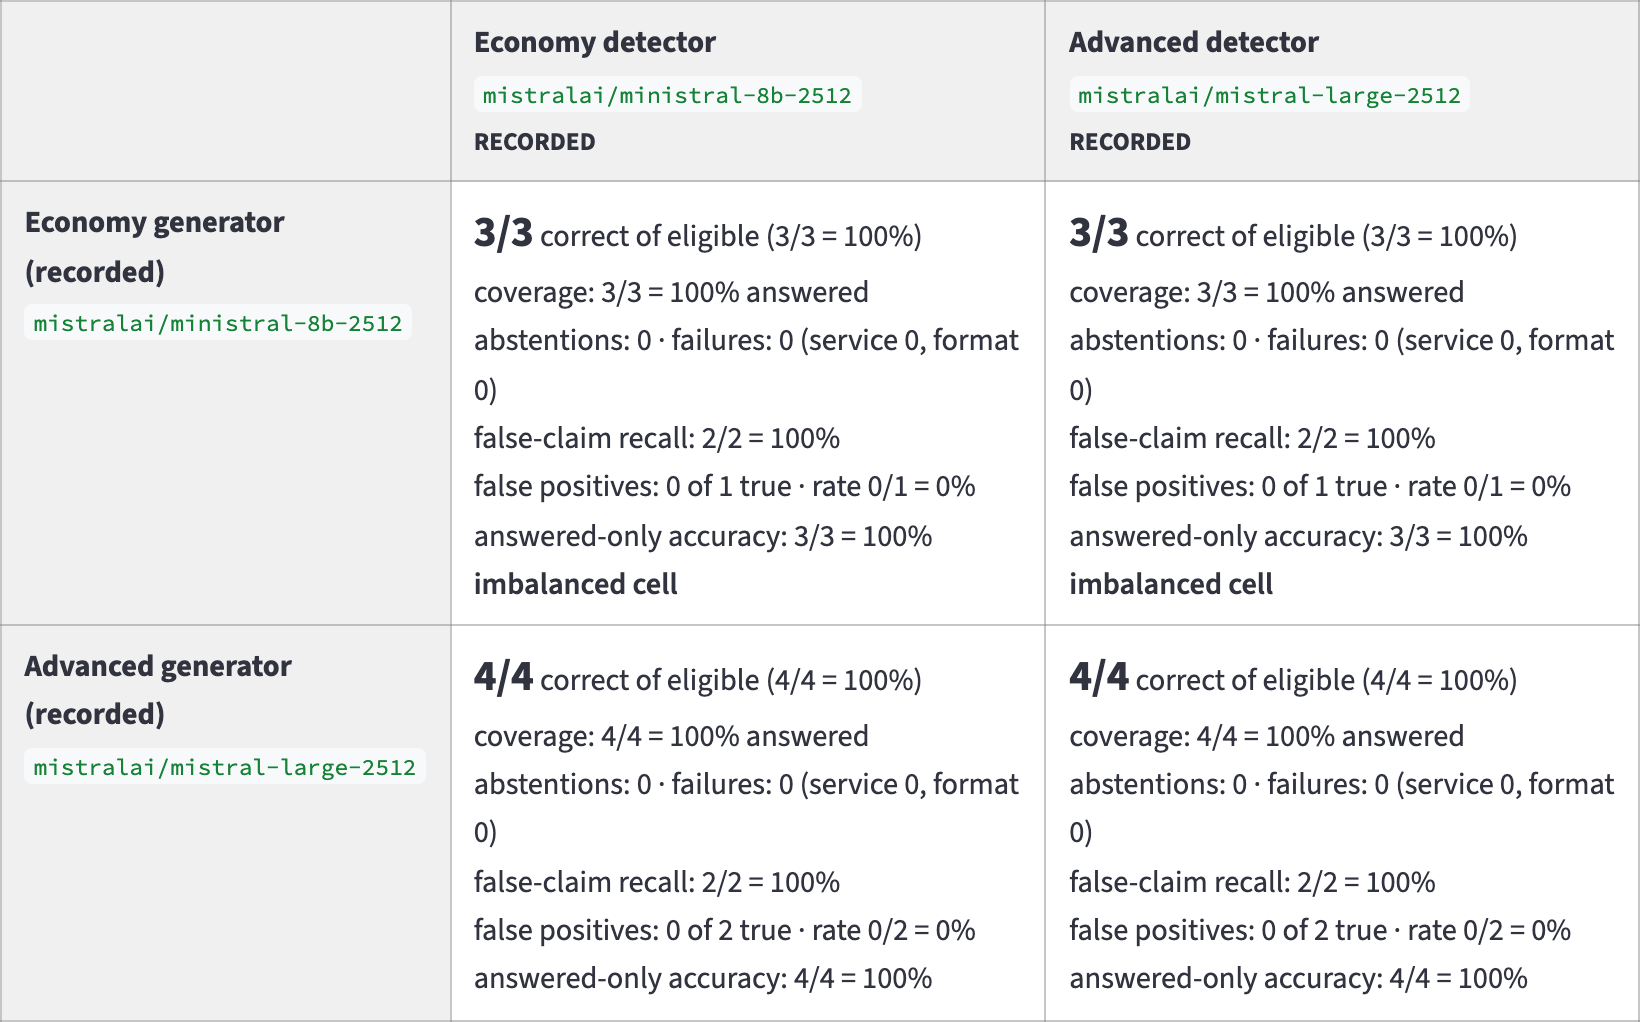
\includegraphics[height=0.78\textheight]{app_matrix.png}
  \slidesource{Screenshot of this app (Detect \& compare tab), recorded rehearsal run of 18 Oct 2026, real model outputs.}
\note{The same numbers as the typeset table in the main part, as the app shows them.}
\end{frame}

% ---- From the source deck (pages 9, 13, 14, 15, 17, 18) ----
\begin{frame}{From the source deck: three families --- one architecture underneath}\label{frm:sourcemap}
  \centering
  \begin{tikzpicture}[x=1mm,y=1mm,
    lane/.style={font=\scriptsize\bfseries, anchor=east},
    dot/.style={circle, fill=accent, minimum size=2.3mm, inner sep=0pt},
    dotg/.style={circle, fill=black!45, minimum size=2.3mm, inner sep=0pt},
    ev/.style={font=\scriptsize, align=flush center, anchor=south, inner sep=1pt}]
    \node[lane, text=accent] at (-2.5,0) {TEXT};
    \node[lane, text=accent] at (-2.5,-11.5) {IMAGES};
    \node[lane, text=accent] at (-2.5,-23) {VIDEO \& VOICE};
    \foreach \y in {0,-11.5,-23}{\draw[black!25, dashed] (0,\y) -- (110,\y);}
    \node[dot] at (24,0) {}; \node[ev] at (24,1.6) {transformer\\(attention)};
    \node[dot] at (66,0) {}; \node[ev] at (66,1.6) {chat assistants};
    \node[dotg] at (2,-11.5) {}; \node[ev, color=black!55] at (4,-9.9) {GANs};
    \node[dot] at (45,-11.5) {}; \node[ev] at (45,-9.9) {diffusion};
    \node[dot] at (66,-11.5) {}; \node[ev] at (66,-9.9) {latent diffusion\\(consumer scale)};
    \node[dot] at (76,-23) {}; \node[ev] at (76,-21.4) {voice cloning\\from 3 seconds};
    \node[dot] at (98,-23) {}; \node[ev] at (98,-21.4) {video with\\native audio};
    \draw[black!30, line width=0.9pt] (0,-29) -- (110,-29);
    \foreach \x/\yr in {2/2014, 24/2017, 45/2020, 66/2022, 87/2024, 108/2026}{
      \draw[black!50] (\x,-30.2) -- (\x,-27.8);
      \node[font=\scriptsize\color{black!55}, anchor=north] at (\x,-30.8) {\yr};}
  \end{tikzpicture}
  \begin{takeaway}[The lanes have converged]
    The 2017 text architecture --- the \emph{transformer} --- now sits inside most new image and video systems too.
  \end{takeaway}
  \slidesource{Source deck p.~9. \textcite{vaswani2017}; \textcite{goodfellow2014}; \textcite{ho2020}; \textcite{rombach2022}; \textcite{chen2025valle}.}
\note{Source slide 9 (map). Today's lecture covers only the text lane. DATES: transformer 2017; GANs 2014;
diffusion made competitive by DDPM 2020; latent diffusion 2022; VALL-E 2023 (preprint; journal 2025);
video with native audio 2025.}
\end{frame}

\begin{frame}{From the source deck: one level deeper --- attention}
  \begin{columns}[T,onlytextwidth]
    \begin{column}{0.54\textwidth}
      \footnotesize
      \begin{itemize}\setlength{\itemsep}{3pt}
        \item \textbf{Embeddings:} each token becomes a vector --- similar meanings end up near each other
        \item \textbf{Self-attention:} every position weighs every earlier one --- ``which words matter here?'' --- all in parallel, which is why it scales
        \item \textbf{Stack + scale:} dozens of such layers, billions of parameters; capability emerges largely from scale
        \item \textbf{Why it matters:} attention gives the model \emph{global context} --- the ingredient of long, coherent, stylistically consistent fakes
      \end{itemize}
    \end{column}
    \begin{column}{0.43\textwidth}
      \centering
      \begin{tikzpicture}[x=1mm,y=1mm]
        \def\cw{6.8}
        \foreach \c/\lab in {0/The, 1/CFO, 2/approved, 3/the, 4/next}{
          \node[font=\scriptsize\color{black!55}, rotate=90, anchor=west, inner sep=0.6pt] at (\c*\cw+\cw/2-1.1, 0.9) {\lab};}
        \foreach \r/\lab in {0/The, 1/CFO, 2/approved, 3/the}{
          \node[font=\scriptsize\color{black!55}, anchor=east, inner sep=0pt] at (-1.8, -\r*\cw-\cw/2+0.6) {\lab};}
        \node[font=\scriptsize\bfseries\color{red!70!black}, anchor=east, inner sep=0pt] at (-1.8, -4*\cw-\cw/2+0.6) {next?};
        \foreach \r/\c/\w in {0/0/90, 1/0/25, 1/1/85, 2/0/15, 2/1/70, 2/2/60, 3/0/20, 3/1/30, 3/2/45, 3/3/40,
                              4/0/10, 4/1/75, 4/2/88, 4/3/22, 4/4/35}{
          \fill[accent, opacity=\w/100, rounded corners=0.5mm] (\c*\cw, -\r*\cw) rectangle (\c*\cw+\cw-1.2, -\r*\cw-\cw+1.2);}
        \draw[red!70!black, line width=0.9pt, rounded corners=1mm] (-0.7,-4*\cw+0.7) rectangle (5*\cw-0.5, -5*\cw+0.5);
      \end{tikzpicture}\\[1mm]
      \parbox{50mm}{\centering\scriptsize\textcolor{red!70!black}{\bfseries The next token leans on ``CFO'' and ``approved''.}\\
      \textcolor{black!55}{Darker = more attention. Illustrative weights.}}
    \end{column}
  \end{columns}
  \slidesource{Source deck p.~13. \textcite{vaswani2017}; attention itself: \textcite{bahdanau2015}.}
\note{Source slide 13. If asked ``wasn't attention older?'': yes --- Bahdanau et al.\ (2015) introduced it
for translation on top of a recurrent network; the 2017 step made self-attention the whole architecture.
Emergence-from-scale is an empirical observation with active debate.}
\end{frame}

\begin{frame}{From the source deck: why the same prompt never gives the same answer}
  {\small The model outputs a distribution --- something still has to \emph{pick}.}\par
  \vspace{2mm}
  \centering
  \begin{tikzpicture}[x=1mm,y=1mm]
    \node[font=\footnotesize\bfseries, anchor=west] at (0,26) {Low ``temperature'' --- safe};
    \foreach \i/\w/\lab in {0/34/payment, 1/9/budget, 2/4/merger, 3/1.5/invoice}{
      \fill[accent!75, rounded corners=0.4mm] (0,20-\i*5.6) rectangle (\w,22.2-\i*5.6);
      \node[font=\scriptsize\color{black!55}, anchor=west] at (\w+1.5,21.1-\i*5.6) {\lab};}
    \node[font=\scriptsize\color{black!55}, anchor=west] at (0,-2.6) {predictable, repetitive --- ``corporate'' prose};
    \node[font=\footnotesize\bfseries, anchor=west] at (66,26) {High ``temperature'' --- creative};
    \foreach \i/\w/\lab in {0/21/payment, 1/16/budget, 2/12/merger, 3/8/invoice}{
      \fill[orange!75, rounded corners=0.4mm] (66,20-\i*5.6) rectangle (66+\w,22.2-\i*5.6);
      \node[font=\scriptsize\color{black!55}, anchor=west] at (66+\w+1.5,21.1-\i*5.6) {\lab};}
    \node[font=\scriptsize\color{black!55}, anchor=west] at (66,-2.6) {surprising, varied --- and more likely to wander};
    \draw[black!25, line width=0.7pt] (59,-5) -- (59,28);
  \end{tikzpicture}
  \vspace{2mm}
  \begin{takeaway}[Governance consequence]
    Output is not reproducible --- ask twice, get two answers. Audit the \emph{logged} output; you may not be able to re-run it.
  \end{takeaway}
  \slidesource{Source deck p.~14. Temperature scales the scores before they become probabilities; see \textcite{holtzman2020}.}
\note{Source slide 14. Even at temperature zero, production systems are only near-deterministic (batching,
hardware). Our app logs every call with its settings for that reason.}
\end{frame}

\begin{frame}{From the source deck: from raw predictor to assistant --- three stages}
  \centering
  \begin{tikzpicture}[x=1mm,y=1mm,
    st/.style={draw=none, rounded corners=1.6mm, align=flush center, inner sep=1.8mm, font=\scriptsize},
    ar/.style={-{Stealth[length=2.2mm]}, line width=0.9pt, color=black!55}]
    \node[st, fill=accent, text=white, text width=40mm, minimum height=16mm] (a) at (0,0)
      {\bfseries 1\; PRETRAINING\\[0.4mm]\mdseries predict the next token,\\over trillions of tokens of text};
    \node[st, fill=accent!25, text width=32mm, minimum height=16mm] (b) at (48,0)
      {\bfseries 2\; INSTRUCTION TUNING\\[0.4mm]\mdseries thousands of\\human-written example answers};
    \node[st, fill=accent!25, text width=32mm, minimum height=16mm] (c) at (92,0)
      {\bfseries 3\; HUMAN FEEDBACK\\[0.4mm]\mdseries people rank answers; the model\\is tuned towards the preferred ones};
    \draw[ar] (a) -- (b); \draw[ar] (b) -- (c);
    \node[font=\scriptsize\color{black!55}, anchor=west] at (-20,-13.5) {relative amount of data:};
    \fill[accent!75, rounded corners=0.4mm] (14,-14.7) rectangle (68,-12.3);
    \fill[accent!35] (68,-14.7) rectangle (70.2,-12.3);
    \node[font=\scriptsize\color{black!55}, anchor=west] at (71.5,-13.5) {stages 2--3: a rounding error};
  \end{tikzpicture}
  \vspace{3mm}
  \begin{columns}[T,onlytextwidth]
    \begin{column}{0.49\textwidth}
      \footnotesize
      \begin{itemize}
        \item Stage 1 buys the \emph{capability} --- the knowledge, the style, the fluency
        \item Stages 2--3 buy the \emph{behaviour} --- helpfulness, tone, refusals
      \end{itemize}
    \end{column}
    \begin{column}{0.49\textwidth}
      \footnotesize
      \begin{itemize}
        \item \textbf{So guardrails are a thin layer over a very general engine --- and ``we fine-tuned it'' is not a safety strategy}
      \end{itemize}
    \end{column}
  \end{columns}
  \slidesource{Source deck p.~15. The classic recipe: \textcite{ouyang2022}. Newer models add further reinforcement-learning stages.}
\note{Source slide 15. InstructGPT: about 13{,}000 written demonstrations (stage 2) and rankings on roughly
33{,}000 prompts (stage 3). There is no separable ``fraud module'' to delete: the same machinery writes the
sales e-mail and the phishing e-mail.}
\end{frame}

\begin{frame}{From the source deck: your turn (Question 1 of 3)}
  \vspace{4mm}
  \begin{exercise}[Question 1 --- discuss or type in the chat]
    \large\textbf{A plausibility engine writes your first draft.}\\[2mm]
    \normalsize Where in \emph{your} studies or work would that be genuinely useful ---
    and where would it be quietly dangerous?\\[2mm]
    Name one of each: \textbf{useful:} \dots\ / \textbf{risky:} \dots
  \end{exercise}
  \vspace{3mm}\centering
  {\footnotesize\color{black!60}No wrong answers --- the next slide shows what the pattern usually is.}
  \slidesource{Source deck p.~17 (optional in this lecture).}
\note{Source slide 17, optional. ``Useful'' answers cluster where a human verifies the output anyway;
``risky'' where output goes out unverified (citations, numbers, legal or medical claims).}
\end{frame}

\begin{frame}{From the source deck: the pattern behind your answers}
  \begin{columns}[T,onlytextwidth]
    \begin{column}{0.49\textwidth}
      \begin{solutionbox}[\faCheck\; Where it is genuinely useful]
        \footnotesize Drafting, summarising, brainstorming, translating, code you are going to run anyway ---
        everything where \emph{a human already checks the output before it matters}.
      \end{solutionbox}
    \end{column}
    \begin{column}{0.49\textwidth}
      \begin{mistake}[\faExclamationTriangle\; Where it is quietly dangerous]
        Citations, numbers, legal or medical claims, anything a customer sees, anything you sign ---
        everything that \emph{ships without a verification step}.
      \end{mistake}
    \end{column}
  \end{columns}
  \vspace{1mm}
  \begin{readme}[The rule worth writing down]
    \footnotesize The risk is not the model --- it is the \emph{missing step} between generation and consequence.
    The same output is excellent in a draft and dangerous in a filing.
    \textbf{So ``don't use AI'' is the wrong policy --- ``never ship unverified output'' is the right one.}
  \end{readme}
  \slidesource{Source deck p.~18. Fabricated citations in court: \textcite{mata2023}.}
\note{Source slide 18; its rule is echoed in takeaway 3 of this lecture.}
\end{frame}

\begin{frame}{Image credits \& licences}\label{frm:credits}
  \footnotesize
  \begin{itemize}\setlength{\itemsep}{3pt}
    \item \textbf{Synthetic face (Round 1A):} ``Woman 1.jpg'' --- StyleGAN2 / thispersondoesnotexist.com output, via Wikimedia Commons, public domain (PD-algorithm).
    \item \textbf{Real portrait (Round 1B):} ``Headshot C.\ Estelle Smith'' by FauxNeme (CC BY-SA 4.0), via Wikimedia Commons; cropped.
    \item \textbf{Arc de Triomphe pair (Round 2):} real: ``Arc de Triomphe de l'\'Etoile at night'' by Wilfredor (CC0); AI: ``Christmas at Arc de Triomphe 2023'' by S\'ergio Valle Duarte via Midjourney (CC BY 3.0), both via Wikimedia Commons.
    \item \textbf{Presenter photograph:} from the author's chapter-00 course deck.
    \item \textbf{App screenshots:} this lecture's Streamlit app, recorded rehearsal run of 18 Oct 2026.
    \item \textbf{Everything else:} original TikZ diagrams, adapted from the source deck.
  \end{itemize}
\note{Keep this slide in any derivative: CC BY / CC BY-SA require attribution. Credits copied from the
source deck's credits slide (p.~36) for the images reused here.}
\end{frame}

\nocite{*}
\begin{frame}[allowframebreaks,t]{References}\label{frm:refs}
  \printbibliography[heading=none]
\end{frame}

% ===================================================== FINAL PAGE (59-60) =====
\section[Resources]{Resources and contact}
\begin{frame}{Resources and contact}\label{frm:resources}
  \begin{labnote}[Course materials from Hochschule Bielefeld (HSBI)]
    \small
    \textbf{AI or Reality? (this lecture)}\hfill{\footnotesize slides, prompts, tested Streamlit app}\\
    \href{https://github.com/ChrisW09/AI-or-Reality}{\color{accent}\faGithub\ \texttt{https://github.com/ChrisW09/AI-or-Reality}}\\[2.5mm]
    \textbf{Python for AI-Driven Automation}\hfill{\footnotesize Python, AI-powered automation, agentic AI}\\
    \href{https://github.com/ChrisW09/Python-for-AI-Driven-Automation}{\color{accent}\faGithub\ \texttt{https://github.com/ChrisW09/Python-for-AI-Driven-Automation}}\\[2.5mm]
    \textbf{Quantitative Research Methods}\hfill{\footnotesize statistical methods, machine learning, quantitative analysis}\\
    \href{https://github.com/ChrisW09/Quantitative-Research-Methods}{\color{accent}\faGithub\ \texttt{https://github.com/ChrisW09/Quantitative-Research-Methods}}
  \end{labnote}
  \vspace{2mm}
  \begin{readme}[Contact]
    \small\textbf{Prof.\ Dr.\ Christoph Weisser} --- Hochschule Bielefeld (HSBI)\hfill
    \faEnvelope[regular]\ \mailme
  \end{readme}
  \vspace{2.5mm}
  \centering{\large Thank you --- questions welcome.}
\note{[59:00--60:00] FINAL PAGE. Leave it on screen: the lecture repository, both course repositories
and the e-mail address are clickable in the PDF. This is the last page of the deck; the appendix sits before it.}
\end{frame}

\end{document}
